\documentclass[11pt,openany]{book}

% ----------------------------------------------------------------------
% Packages
% ----------------------------------------------------------------------
\usepackage[T1]{fontenc}
\usepackage{lmodern}
\usepackage[utf8]{inputenc}
\usepackage[margin=1in]{geometry}
\usepackage{amsmath,amssymb,amsthm,mathtools}
\usepackage{graphicx}
\usepackage{xcolor}
\usepackage{booktabs}
\usepackage{array}
\usepackage{enumitem}
\usepackage{microtype}
\usepackage{tikz}
\usetikzlibrary{arrows.meta,positioning,shapes.geometric,calc}
\usepackage[most]{tcolorbox}
\usepackage{titlesec}
\usepackage{fancyhdr}
\usepackage[hidelinks]{hyperref}
\usepackage{caption}

\captionsetup{font=small,labelfont=bf,labelsep=period}
\graphicspath{{figures/}}

% ----------------------------------------------------------------------
% Colors
% ----------------------------------------------------------------------
\definecolor{accent}{HTML}{1F5FA8}
\definecolor{accentdark}{HTML}{16406F}
\definecolor{accentlight}{HTML}{EAF1FA}
\definecolor{exgreen}{HTML}{2A8F5A}
\definecolor{exgreenlight}{HTML}{EAF5EF}
\definecolor{warmred}{HTML}{B03030}
\definecolor{goldline}{HTML}{C9A227}
\definecolor{softgrey}{HTML}{F4F4F4}

% ----------------------------------------------------------------------
% Theorem-like environments
% ----------------------------------------------------------------------
\theoremstyle{definition}
\newtheorem{definition}{Definition}[chapter]
\newtheorem{principle}[definition]{Principle}
\newtheorem{remark}[definition]{Remark}

\theoremstyle{plain}
\newtheorem{theorem}[definition]{Theorem}
\newtheorem{proposition}[definition]{Proposition}
\newtheorem{lemma}[definition]{Lemma}
\newtheorem{corollary}[definition]{Corollary}

% Boxed "key idea" definition
\newtcolorbox{keybox}[1][]{
  enhanced, breakable, colback=accentlight, colframe=accent,
  boxrule=0.8pt, arc=2pt, left=8pt, right=8pt, top=6pt, bottom=6pt,
  fonttitle=\bfseries\color{white},
  coltitle=white, attach boxed title to top left={xshift=8pt,yshift=-2pt},
  boxed title style={colback=accent,arc=1pt}, #1}

% Example environment (counter per chapter)
\newcounter{example}[chapter]
\renewcommand{\theexample}{\thechapter.\arabic{example}}

\newtcolorbox{exbox}[1][]{
  enhanced, breakable, colback=exgreenlight, colframe=exgreen,
  boxrule=0.7pt, arc=2pt, left=7pt, right=7pt, top=5pt, bottom=6pt,
  before skip=10pt, after skip=10pt,
  borderline west={3pt}{0pt}{exgreen},
  #1}

% \begin{example}{title} ... \end{example}
\newenvironment{example}[1][]{%
  \refstepcounter{example}%
  \begin{exbox}%
  {\bfseries\color{exgreen}Example~\theexample}%
  \ifx\\#1\\\else\ \textbf{(#1)}\fi\par\smallskip\noindent\ignorespaces}{%
  \end{exbox}}

% Solution marker
\newcommand{\solution}{\par\smallskip\noindent\textit{\color{accentdark}Solution.}\ \ignorespaces}

% ----------------------------------------------------------------------
% Section / chapter styling
% ----------------------------------------------------------------------
\titleformat{\chapter}[display]
  {\normalfont\huge\bfseries\color{accentdark}}
  {\filright\large\color{accent}\MakeUppercase{\chaptertitlename}\ \thechapter}
  {6pt}{\Huge}
\titlespacing*{\chapter}{0pt}{6pt}{22pt}

\titleformat{\section}
  {\normalfont\Large\bfseries\color{accentdark}}{\thesection}{0.6em}{}
\titleformat{\subsection}
  {\normalfont\large\bfseries\color{accent}}{\thesubsection}{0.6em}{}

\setlength{\parskip}{0.45em}
\setlength{\parindent}{0pt}

% Header / footer
\pagestyle{fancy}
\fancyhf{}
\renewcommand{\headrulewidth}{0.4pt}
\fancyhead[L]{\small\itshape\nouppercase{\leftmark}}
\fancyhead[R]{\small\thepage}

% ----------------------------------------------------------------------
% Math shortcuts
% ----------------------------------------------------------------------
\newcommand{\E}{\mathbb{E}}
\newcommand{\Var}{\mathrm{Var}}
\newcommand{\Cov}{\mathrm{Cov}}
\newcommand{\R}{\mathbb{R}}
\newcommand{\given}{\,|\,}
\newcommand{\Prob}{\mathbb{P}}
\newcommand{\Ber}{\mathrm{Ber}}
\newcommand{\Bin}{\mathrm{Bin}}
\newcommand{\Geo}{\mathrm{Geo}}
\newcommand{\Pois}{\mathrm{Pois}}
\newcommand{\Exp}{\mathrm{Exp}}
\newcommand{\Unif}{\mathrm{Unif}}
\newcommand{\Mult}{\mathrm{Mult}}
\newcommand{\Par}{\mathrm{Par}}
\newcommand{\N}{\mathcal{N}}
\newcommand{\xbar}{\bar{x}}
\newcommand{\ybar}{\bar{y}}
\newcommand{\Xbar}{\bar{X}}
\newcommand{\Ybar}{\bar{Y}}
\newcommand{\eqdef}{\vcentcolon=}
\DeclareMathOperator{\Med}{Med}
\DeclareMathOperator{\MAD}{MAD}
\DeclareMathOperator*{\argmax}{arg\,max}
\DeclareMathOperator*{\argmin}{arg\,min}

% ----------------------------------------------------------------------
\begin{document}
\frontmatter

% ===================== TITLE PAGE =====================
\begin{titlepage}
\centering
\vspace*{1.5cm}
{\color{accent}\rule{\linewidth}{1.5pt}}\par
\vspace{0.8cm}
{\Huge\bfseries\color{accentdark} Probability \& Statistics}\par
\vspace{0.4cm}
{\LARGE\color{accent} Lecture Notes with Worked Examples}\par
\vspace{0.5cm}
{\large A One-Semester Course}\par
\vspace{0.4cm}
{\color{accent}\rule{\linewidth}{1.5pt}}\par
\vspace{1.6cm}

\begin{tikzpicture}[scale=1.0]
  % a small decorative normal curve + scatter motif
  \begin{scope}
  \draw[accent,line width=1pt] plot[domain=-3:3,samples=80]
     (\x, {2.2*exp(-\x*\x/2)});
  \draw[->,gray] (-3.4,0)--(3.4,0);
  \fill[warmred] (-1,0.05) circle (1pt) (0.4,0.05) circle(1pt)
     (1.6,0.05) circle(1pt) (-0.3,0.05) circle(1pt) (2.1,0.05) circle(1pt)
     (-2,0.05) circle(1pt) (0.9,0.05) circle(1pt);
  \end{scope}
\end{tikzpicture}

\vspace{1.6cm}
{\large A unified treatment of exploratory data analysis, probability,\\[2pt]
statistical inference, maximum likelihood, regression,\\[2pt]
and goodness-of-fit testing.}\par
\vfill
{\large Course notes and integrated problem set}\par
\vspace{0.3cm}
{\color{accent}\rule{0.5\linewidth}{0.8pt}}
\end{titlepage}

% ===================== PREFACE =====================
\chapter*{About These Notes}
\addcontentsline{toc}{chapter}{About These Notes}
\markboth{About These Notes}{About These Notes}

These notes assemble the material of a one-semester introductory course in
probability and statistics into a single self-contained volume. The aim is to
present the theory and a large stock of fully worked examples \emph{side by
side}, so that every idea is immediately illustrated by concrete computation.

The book is organized into three movements. The first
(Chapters~\ref{ch:prereq}--\ref{ch:limits}) develops the language of
probability: sets and counting, conditional probability and Bayes' rule,
discrete and continuous random variables, joint distributions, and the
classical limit theorems. The second (Chapter~\ref{ch:eda}) turns to data
itself through exploratory data analysis. The third
(Chapters~\ref{ch:inference}--\ref{ch:gof}) builds the machinery of
statistical inference: point estimation, confidence intervals, maximum
likelihood, least-squares regression, and hypothesis testing culminating in
goodness-of-fit tests.

Every worked example is woven into the section whose ideas it exercises. A
problem about joint distributions appears beside the discussion of joint
distributions; a maximum-likelihood computation appears beside the maximum
likelihood principle. Where the original course used the statistical
software \textsf{R} for computation, the corresponding numerical answers are
simply stated, since the emphasis here is on the underlying reasoning rather
than on software commands.

A short note on figures: the plots in these notes were regenerated from the
underlying datasets (the black cherry tree volumes, the town mortality and
calcium measurements, and the small numerical datasets that appear in the
examples). The Old Faithful illustrations use a dataset constructed to match
the summary statistics quoted in the text and are meant to be illustrative.

\tableofcontents

\mainmatter

\chapter{Mathematical Prerequisites}
\label{ch:prereq}

Probability and statistics lean heavily on a handful of tools from calculus.
Expectations of continuous random variables are integrals; the maximum
likelihood method finds estimates by differentiating and setting the
derivative to zero; tail probabilities are computed by integrating density
functions. Before we begin, this short chapter revisits the differentiation
and integration techniques that recur throughout the book. A reader fluent in
single-variable calculus may skip directly to Chapter~\ref{ch:probability} and
refer back as needed.

\section{Differentiation}

The two rules we use most often are the \emph{product rule}
\[
  \frac{d}{dx}\bigl(u(x)\,v(x)\bigr) = u'(x)\,v(x) + u(x)\,v'(x)
\]
and the \emph{chain rule}
\[
  \frac{d}{dx}\,f\bigl(g(x)\bigr) = f'\bigl(g(x)\bigr)\,g'(x).
\]
Together with the quotient rule and the elementary derivatives of $e^x$,
$\ln x$, and the trigonometric functions, these handle essentially every
derivative that arises in this course.

\begin{example}
Differentiate $f(x) = x^2 \ln x$.

\solution The function is a product, so the product rule with $u=x^2$ and
$v=\ln x$ gives
\[
  f'(x) = (2x)\ln x + x^2\cdot\frac{1}{x} = 2x\ln x + x.
\]
\end{example}

\begin{example}
Let $f(x) = x e^{-x}$. Find $f'(x)$ and $f''(x)$.

\solution Applying the product rule once,
\[
  f'(x) = e^{-x} + x(-e^{-x}) = e^{-x} - xe^{-x}.
\]
Differentiating again, and reusing the result just obtained for the second
term,
\[
  f''(x) = -e^{-x} - \bigl(e^{-x} - xe^{-x}\bigr)
         = -2e^{-x} + xe^{-x}.
\]
This particular function reappears when we study the gamma-type densities and
integration by parts.
\end{example}

\begin{example}
Differentiate $y = e^{-(x-1)^2/2}$.

\solution This is a composition, so we peel it apart with the chain rule. The
outer function is $e^{u}$ with $u = -\tfrac12(x-1)^2$, and $u' = -(x-1)$. Hence
\[
  \frac{dy}{dx} = e^{-(x-1)^2/2}\cdot\bigl(-(x-1)\bigr)
              = -(x-1)\,e^{-(x-1)^2/2}.
\]
The exponent here is precisely the kernel of the standard normal density,
which is why this derivative shows up when we maximize normal likelihoods.
\end{example}

\section{Integration}

The reverse operation, integration, computes areas and—crucially for us—the
expectations and probabilities of continuous random variables. We use basic
antiderivatives, linearity, the substitution rule, and integration by parts.

\subsection{Antiderivatives and definite integrals}

\begin{example}
Evaluate $\displaystyle\int\!\left(x^3 + e^x\right)dx$ and
$\displaystyle\int\!\left(2\theta + \tfrac{1}{\theta}\right)d\theta$.

\solution Integrating term by term,
\[
  \int\!\left(x^3 + e^x\right)dx = \frac{x^4}{4} + e^x + C,
  \qquad
  \int\!\left(2^\theta + \tfrac{1}{\theta}\right)d\theta
     = \frac{2^\theta}{\ln 2} + \ln|\theta| + C.
\]
(The exponential $2^\theta$ has antiderivative $2^\theta/\ln 2$ because
$\frac{d}{d\theta}2^\theta = 2^\theta\ln 2$.)
\end{example}

\begin{example}
Evaluate the definite integral $\displaystyle\int_0^{\pi/2} -2\cos\theta\,d\theta$.

\solution An antiderivative of $-2\cos\theta$ is $-2\sin\theta$, so
\[
  \int_0^{\pi/2} -2\cos\theta\,d\theta
     = \bigl[-2\sin\theta\bigr]_0^{\pi/2}
     = -2\sin(\tfrac{\pi}{2}) + 2\sin 0 = -2.
\]
\end{example}

\subsection{Integration by parts}

The integration-by-parts formula,
\[
  \int u\,dv = uv - \int v\,du,
\]
is indispensable for computing expectations of the form $\int x f(x)\,dx$ when
$f$ involves an exponential. We will use it repeatedly—for instance to show
that an $\Exp(\lambda)$ random variable has mean $1/\lambda$, and that the
square of a standard normal random variable has expectation $1$.

\begin{example}
Use integration by parts to evaluate
$\displaystyle\int_0^\infty x\,\lambda e^{-\lambda x}\,dx$ for $\lambda > 0$.

\solution Take $u = x$ and $dv = \lambda e^{-\lambda x}\,dx$, so that
$du = dx$ and $v = -e^{-\lambda x}$. Then
\[
  \int_0^\infty x\,\lambda e^{-\lambda x}\,dx
    = \Bigl[-xe^{-\lambda x}\Bigr]_0^\infty + \int_0^\infty e^{-\lambda x}\,dx
    = 0 + \left[-\frac{1}{\lambda}e^{-\lambda x}\right]_0^\infty
    = \frac{1}{\lambda}.
\]
This is exactly the mean of an exponential random variable with rate
$\lambda$, a fact we will meet again in Chapter~\ref{ch:continuous}.
\end{example}

With these tools in hand we are ready to build the theory of probability.

\chapter{The Language of Probability}
\label{ch:probability}

Probability theory is a precise language for reasoning about uncertainty. Its
basic objects are \emph{experiments} whose outcomes cannot be predicted with
certainty, and its goal is to assign numbers—probabilities—to the various
things that might happen. This chapter introduces that language: sample
spaces and events, the rules probabilities must obey, counting, and the
profoundly useful ideas of conditional probability, independence, and Bayes'
theorem.

\section{Sample Spaces and Events}

The set of all possible outcomes of an experiment is the \emph{sample space},
denoted $\Omega$. An \emph{event} is a subset of $\Omega$: a collection of
outcomes we might be interested in. Because events are sets, the operations of
set theory—union ($\cup$, ``or''), intersection ($\cap$, ``and''), and
complement ($A^c$, ``not'')—are exactly the operations we use to combine and
negate events.

\begin{example}
A coin is tossed three times, recording heads (H) or tails (T) each time, so
\[
  \Omega = \{HHH,\,THH,\,HTH,\,HHT,\,TTH,\,THT,\,HTT,\,TTT\}.
\]
Consider the events
$A=$``exactly two tails,''
$B=$``at least two tails,''
$C=$``no head precedes the first tail'' (equivalently, tails never appears
after a head),
and $D=$``the first toss is tails.''
Express $A,B,C,D$ as sets, and then find $A^c$, $A\cup(C\cap D)$, and
$A\cap D^c$.

\solution Reading off the outcomes,
\[
  A=\{TTH,THT,HTT\},\quad
  B=\{TTH,THT,HTT,TTT\},
\]
\[
  C=\{HHH,HHT,HTT,TTT\},\quad
  D=\{THH,TTH,THT,TTT\}.
\]
The complement of $A$ contains every outcome that is \emph{not} in $A$:
\[
  A^c=\{HHH,THH,HTH,HHT,TTT\}.
\]
Since $C\cap D=\{TTT\}$ (the only outcome in both), we have
$A\cup(C\cap D)=\{TTT,TTH,THT,HTT\}$. Finally $D^c=\{HHH,HTH,HHT,HTT\}$, and the
only outcome common to $A$ and $D^c$ is $HTT$, so $A\cap D^c=\{HTT\}$.
\end{example}

Sometimes it is the \emph{structure} of the experiment, rather than an explicit
list, that tells us what the sample space should be.

\begin{example}
A coin with $\Prob(\text{heads})=p$ is tossed repeatedly until heads appears for
the \emph{second} time. What is a natural sample space, and what is the
probability that exactly five tosses are required?

\solution The quantity of interest is the toss on which the second head lands;
this is at least $2$, so $\Omega=\{2,3,4,\dots\}$. For the second head to occur
on toss $5$, exactly one of the first four tosses is a head and the fifth is a
head. There are four positions for that early head, each sequence having
probability $p^2(1-p)^3$, so the answer is
\[
  4\,p^2(1-p)^3. \qedhere
\]
\end{example}

\section{The Rules of Probability}

A probability assignment must satisfy a few axioms: every event has probability
between $0$ and $1$, the whole sample space has probability $1$, and the
probability of a union of \emph{disjoint} events is the sum of their
probabilities. From these follow the rules we use constantly. The most
important is the \emph{addition rule} (inclusion--exclusion for two events):
\[
  \Prob(A\cup B)=\Prob(A)+\Prob(B)-\Prob(A\cap B).
\]
The subtracted term corrects for the overlap, which would otherwise be counted
twice.

\begin{example}
Suppose $\Prob(A)=\tfrac23$, $\Prob(B)=\tfrac16$, and $\Prob(A\cap B)=\tfrac19$.
Find $\Prob(A\cup B)$.

\solution By the addition rule,
\[
  \Prob(A\cup B)=\tfrac23+\tfrac16-\tfrac19
   =\tfrac{12}{18}+\tfrac{3}{18}-\tfrac{2}{18}=\tfrac{13}{18}. \qedhere
\]
\end{example}

\begin{example}
For events with $\Prob(A)=0.4$, $\Prob(B)=0.5$, and $\Prob(A\cap B)=0.1$, find
the probability that \emph{exactly one} of $A$, $B$ occurs.

\solution ``$A$ or $B$ but not both'' is the event $A\cup B$ with the overlap
removed. Since $\Prob(A\cup B)=0.4+0.5-0.1=0.8$, the probability of exactly one
is
\[
  \Prob(A\cup B)-\Prob(A\cap B)=0.8-0.1=0.7. \qedhere
\]
\end{example}

The addition rule also lets us \emph{bound} probabilities even when we do not
know the overlap exactly.

\begin{example}
Two disasters $D_1$ and $D_2$ are each rare: $\Prob(D_1)\le 10^{-6}$ and
$\Prob(D_2)\le 10^{-6}$. What can be said about the probability that at least
one occurs, and that both occur?

\solution Because probabilities are nonnegative, dropping the (subtracted)
intersection term can only increase the bound:
\[
  \Prob(D_1\cup D_2)=\Prob(D_1)+\Prob(D_2)-\Prob(D_1\cap D_2)
   \le 10^{-6}+10^{-6}=2\times10^{-6}.
\]
For the intersection, note $D_1\cap D_2\subseteq D_1$, so monotonicity gives
$\Prob(D_1\cap D_2)\le\Prob(D_1)\le 10^{-6}$.
\end{example}

\section{Counting}

When every outcome of a finite experiment is equally likely, computing a
probability reduces to counting: $\Prob(A)$ is the number of outcomes in $A$
divided by the total number of outcomes. The binomial coefficient
$\binom{n}{k}=\frac{n!}{k!\,(n-k)!}$ counts the number of ways to choose $k$
items from $n$ without regard to order.

\begin{example}
A system has five components, each either working ($1$) or failed ($0$), so an
outcome is a vector $(x_1,\dots,x_5)$. In how many ways can it happen that
exactly two components work and three have failed?

\solution We must choose which $2$ of the $5$ positions hold a $1$; the rest are
$0$. The number of such choices is $\binom{5}{2}=10$. (Explicitly, the ten
outcomes range from $(1,1,0,0,0)$ through $(0,0,0,1,1)$.)
\end{example}

\section{Conditional Probability and Independence}

The \emph{conditional probability} of $A$ given $B$ rescales probabilities to
the world in which $B$ is known to have occurred:
\[
  \Prob(A\given B)=\frac{\Prob(A\cap B)}{\Prob(B)},\qquad \Prob(B)\neq 0.
\]
Two events are \emph{independent} if knowing one tells us nothing about the
other—formally, if $\Prob(A\cap B)=\Prob(A)\Prob(B)$, equivalently
$\Prob(A\given B)=\Prob(A)$.

\begin{example}
A fair die is thrown twice. Let $A$ be ``the two throws sum to $4$'' and $B$ be
``at least one throw is a $3$.'' Compute $\Prob(A\given B)$, and decide whether
$A$ and $B$ are independent.

\solution Event $B$ consists of the eleven equally likely outcomes containing a
$3$. Of these, only $(1,3)$ and $(3,1)$ sum to $4$, so
$\Prob(A\given B)=\tfrac{2}{11}$. For independence, compare: $A=\{(1,3),(3,1),(2,2)\}$
has $\Prob(A)=\tfrac{3}{36}=\tfrac1{12}$, which is \emph{not} equal to
$\Prob(A\given B)=\tfrac2{11}$. The events are therefore dependent.
\end{example}

Independence makes ``and'' probabilities multiply, which is what lets us model
repeated trials.

\begin{example}
Two laboratory experiments are run each day in separate rooms, independently,
until at least one succeeds; each succeeds with probability $p$. What is the
probability that the first success occurs on day $n$?

\solution On any single day the probability that \emph{at least one} room
succeeds is, by the addition rule and independence,
\[
  q \eqdef \Prob(\text{success on a given day}) = p+p-p^2 = 2p-p^2.
\]
Reaching day $n$ with the first success requires $n-1$ failed days followed by a
successful one. Since days are independent,
\[
  \Prob(\text{first success on day }n) = (1-q)^{\,n-1}q
   = \bigl(1-(2p-p^2)\bigr)^{n-1}(2p-p^2). \qedhere
\]
\end{example}

\section{The Law of Total Probability and Bayes' Theorem}

Often we know the probability of an event \emph{conditional} on each of several
scenarios, and want the overall probability. The \emph{law of total
probability} stitches the scenarios together: if $B$ and $B^c$ partition the
sample space,
\[
  \Prob(A)=\Prob(A\given B)\Prob(B)+\Prob(A\given B^c)\Prob(B^c).
\]
Reversing the direction of conditioning is the job of \emph{Bayes' theorem}:
\[
  \Prob(B\given A)=\frac{\Prob(A\given B)\,\Prob(B)}{\Prob(A)}
   =\frac{\Prob(A\given B)\Prob(B)}{\Prob(A\given B)\Prob(B)+\Prob(A\given B^c)\Prob(B^c)}.
\]
This is the workhorse of medical testing, reliability, and inference. The
following examples show its range.

\begin{example}[Diagnostic test for a rare condition]
A cow is tested for BSE with sensitivity $\Prob(T\given B)=0.70$ and
false-positive rate $\Prob(T\given B^c)=0.10$, where $B$ is ``the cow is
infected'' and $T$ is ``the test is positive.'' The prevalence is
$\Prob(B)=1.3\times10^{-5}$. Find $\Prob(B\given T)$.

\solution Bayes' theorem with the law of total probability in the denominator
gives
\[
  \Prob(B\given T)=\frac{0.70\,(1.3\times10^{-5})}
   {0.70\,(1.3\times10^{-5})+0.10\,(1-1.3\times10^{-5})}\approx 9\times10^{-5}.
\]
Even after a positive test the cow is almost certainly healthy: when a
condition is extremely rare, false positives vastly outnumber true positives.
This counterintuitive phenomenon is the \emph{base-rate} effect.
\end{example}

\begin{example}[Solving for the test quality]
A breath analyzer satisfies $\Prob(A\given B)=\Prob(A^c\given B^c)=p$, where $A$
is ``the analyzer reports over the limit'' and $B$ is ``the driver is truly over
the limit.'' On a Saturday night, $5\%$ of drivers are over the limit. How
large must $p$ be so that $\Prob(B\given A)=0.9$?

\solution By Bayes' theorem,
\[
  0.9=\Prob(B\given A)=\frac{p(0.05)}{p(0.05)+(1-p)(0.95)}.
\]
Clearing the denominator,
$0.9\bigl(0.05p+0.95(1-p)\bigr)=0.05p$, which rearranges to
$\bigl(\tfrac{0.05}{0.9}+0.9\bigr)p=0.95$, giving $p\approx 0.994$. A very
accurate device is needed before a positive reading is convincing, again
because the underlying event is uncommon.
\end{example}

\begin{example}[Two independent tests]
A disease has prevalence $\Prob(D)=0.01$. A test satisfies $\Prob(T\given D)=0.98$
and $\Prob(T^c\given D^c)=0.95$. (a)~Given one positive test, find
$\Prob(D\given T)$. (b)~A second, independent test also comes back positive; now
find $\Prob(D\given T_1\cap T_2)$.

\solution (a)~Bayes' theorem yields
\[
  \Prob(D\given T)=\frac{0.98(0.01)}{0.98(0.01)+0.05(0.99)}
   =\frac{0.0098}{0.0593}\approx 0.166.
\]
(b)~The two tests are independent \emph{conditional on disease status}, so
\begin{align*}
  \Prob(D\given T_1\cap T_2)
   &=\frac{\Prob(T_1\given D)\Prob(T_2\given D)\Prob(D)}
   {\Prob(T_1\given D)\Prob(T_2\given D)\Prob(D)+\Prob(T_1\given D^c)\Prob(T_2\given D^c)\Prob(D^c)}\\[4pt]
   &=\frac{(0.98)^2(0.01)}{(0.98)^2(0.01)+(0.05)^2(0.99)}\approx 0.795.
\end{align*}
\emph{A subtle point.} It is tempting to write
$\Prob(T_1\cap T_2)=\Prob(T_1)\Prob(T_2)$, but that is wrong: the tests are
\emph{not} unconditionally independent. They are independent only once disease
status is fixed. Indeed a first positive raises the chance of disease, which in
turn raises the chance the second test is positive. This distinction—between
independence and \emph{conditional} independence—is one of the most important
in all of probability.
\end{example}

\begin{example}[A multiple-choice exam]
On each question a student either knows the answer (then answers correctly with
probability $1$) or guesses among the options (then correct with probability
$\tfrac14$). The student knows each answer with probability $0.6$. Given that a
question is answered correctly, what is the probability the student actually
knew it?

\solution Let $B=$``knows the answer,'' $A=$``answers correctly.'' Then
$\Prob(B)=0.6$, $\Prob(A\given B)=1$, $\Prob(A\given B^c)=\tfrac14$, and Bayes'
theorem gives
\[
  \Prob(B\given A)=\frac{1\cdot 0.6}{1\cdot 0.6 + \tfrac14\cdot 0.4}
   =\frac{0.6}{0.7}=\frac{6}{7}. \qedhere
\]
\end{example}

\begin{example}[The neighbor and the plant]
While you are away, a neighbor waters a sickly plant. Without water it dies with
probability $0.8$; with water it dies with probability $0.15$. You are $90\%$
sure the neighbor remembers. (a)~Find the probability the plant is alive on your
return. (b)~If it is dead, find the probability the neighbor forgot.

\solution Let $A=$``alive'' and $R=$``remembers to water.'' By the law of total
probability,
\[
  \Prob(A)=\Prob(A\given R)\Prob(R)+\Prob(A\given R^c)\Prob(R^c)
   =(0.85)(0.9)+(0.2)(0.1)=\tfrac{157}{200}.
\]
For part (b), Bayes' theorem with $A^c$ gives
\[
  \Prob(R^c\given A^c)=\frac{\Prob(A^c\given R^c)\Prob(R^c)}{\Prob(A^c)}
   =\frac{(0.8)(0.1)}{1-\tfrac{157}{200}}=\frac{0.08}{43/200}=\frac{16}{43}. \qedhere
\]
\end{example}

\begin{example}[Inferring an infestation from a union]
Grapefruit is grown in two regions, $R_1$ and $R_2$. Let $A$ and $B$ be the
events that $R_1$ and $R_2$ respectively are infested with a parasite, with
$\Prob(A)=\tfrac34$, $\Prob(B)=\tfrac25$, and $\Prob(A\cup B)=\tfrac45$. If a
shipment from $R_1$ is found infested, what is the probability $R_2$ is infested
too?

\solution We want $\Prob(B\given A)=\Prob(A\cap B)/\Prob(A)$. The addition rule
recovers the intersection:
$\Prob(A\cap B)=\Prob(A)+\Prob(B)-\Prob(A\cup B)=\tfrac34+\tfrac25-\tfrac45=\tfrac{7}{20}$.
Hence $\Prob(B\given A)=\tfrac{7/20}{3/4}=\tfrac{7}{15}$.
\end{example}

\subsection{Bayes' theorem with geometric structure: the three-card problem}

\begin{example}[Three cards]
Three cards are placed in a hat: one green on both sides, one red on both sides,
and one green on one side and red on the other. You draw a card and look at one
side, both chosen at random. The side you see is green. What is the probability
the other side is also green?

\solution Let $G_1$ be ``the visible side is green'' and $G_2$ be ``the hidden
side is green.'' The only way \emph{both} sides are green is the green--green
card, so $\Prob(G_1\cap G_2)=\tfrac13$. By symmetry $\Prob(G_1)=\tfrac12$ (half
of all six card-faces are green). Therefore
\[
  \Prob(G_2\given G_1)=\frac{\Prob(G_1\cap G_2)}{\Prob(G_1)}
   =\frac{1/3}{1/2}=\frac{2}{3}.
\]
The intuitive guess of $\tfrac12$ is wrong: seeing a green face makes the
double-green card more likely than the mixed card, because the double-green card
has \emph{two} ways to show you a green face.
\end{example}

\subsection{The Monty Hall problem}

\begin{example}[Monty Hall]
A car sits behind one of three doors; goats sit behind the other two. You pick a
door, and the host—who knows where the car is—opens a different door to reveal a
goat. Should you switch? Label the door hiding the car $a$ and the others $b,c$,
and model the experiment by the product space $\Omega=\{a,b,c\}\times\{a,b,c\}$,
where the first coordinate is your choice and the second is the door the host
opens.

\solution The host never opens door $a$ (the car is there), so any pair with
second coordinate $a$ has probability $0$. If you pick $a$ (probability
$\tfrac13$), the host chooses $b$ or $c$ equally, giving
$\Prob((a,b))=\Prob((a,c))=\tfrac13\cdot\tfrac12=\tfrac16$. If you pick $b$, the
host must open $c$, so $\Prob((b,c))=\tfrac13$; similarly $\Prob((c,b))=\tfrac13$.

A \emph{no-switch} player wins exactly when the original pick is $a$, an event of
probability $\tfrac16+\tfrac16=\tfrac13$. A \emph{switching} player wins exactly
when the original pick was $b$ or $c$, namely on $\{(b,c),(c,b)\}$, of
probability $\tfrac13+\tfrac13=\tfrac23$. Switching doubles your chances.
\end{example}

\begin{center}
\begin{tikzpicture}[font=\small,>=Stealth, level distance=15mm,
   level 1/.style={sibling distance=34mm},
   level 2/.style={sibling distance=15mm}]
\node[circle,draw=accent,fill=accentlight,inner sep=1.5pt] {pick}
  child {node[draw,rounded corners,fill=softgrey] {pick $a$ ($\tfrac13$)}
    child {node {host $b$} edge from parent node[left,font=\tiny]{$\tfrac12$}}
    child {node {host $c$} edge from parent node[right,font=\tiny]{$\tfrac12$}}}
  child {node[draw,rounded corners,fill=softgrey] {pick $b$ ($\tfrac13$)}
    child {node {host $c$} edge from parent node[right,font=\tiny]{$1$}}}
  child {node[draw,rounded corners,fill=softgrey] {pick $c$ ($\tfrac13$)}
    child {node {host $b$} edge from parent node[right,font=\tiny]{$1$}}};
\end{tikzpicture}
\captionof{figure}{The Monty Hall experiment. Staying wins only on the left
branch (probability $\tfrac13$); switching wins on the other two
(probability $\tfrac23$).}
\end{center}

\chapter{Discrete Random Variables}
\label{ch:discrete}

A \emph{random variable} is a numerical summary of the outcome of an
experiment—a function that assigns a number to each point of the sample space.
A random variable is \emph{discrete} when it takes values in a finite or
countable set, such as the number of heads in ten tosses or the number of
trials until a success. This chapter develops the standard discrete models and
the two numbers—expectation and variance—that summarize them.

\section{Probability Mass and Distribution Functions}

The \emph{probability mass function} (pmf) of a discrete random variable $X$ is
$p_X(a)=\Prob(X=a)$. It is nonnegative and sums to one over the possible values.
The \emph{cumulative distribution function} (cdf) accumulates the mass,
$F_X(a)=\Prob(X\le a)$, and is a nondecreasing step function that rises from $0$
to $1$.

\section{Expectation and Variance}

The \emph{expectation} (or mean) of $X$ is the probability-weighted average of
its values,
\[
  \E[X]=\sum_a a\,p_X(a),
\]
and the \emph{variance} measures spread about the mean,
\[
  \Var(X)=\E\bigl[(X-\E[X])^2\bigr]=\E[X^2]-(\E[X])^2.
\]
The second form on the right is almost always the easier one to compute.
Expectation is \emph{linear}: $\E[aX+bY]=a\E[X]+b\E[Y]$ for any random variables
and constants, whether or not $X$ and $Y$ are independent.

\begin{example}[A fair four-sided die]
A four-sided die shows $X\in\{1,2,3,4\}$, each with probability $\tfrac14$.
Compute $\E[X]$ and $\Var(X)$.

\solution The mean is
\[
  \E[X]=\tfrac14(1+2+3+4)=\tfrac{10}{4}=\tfrac52.
\]
For the variance, first $\E[X^2]=\tfrac14(1+4+9+16)=\tfrac{30}{4}$, so
\[
  \Var(X)=\E[X^2]-(\E[X])^2=\tfrac{30}{4}-\tfrac{25}{4}=\tfrac54. \qedhere
\]
\end{example}

\subsection{Functions of a discrete random variable}

To find the distribution of $Y=g(X)$, we collect the probability of each value
of $X$ onto the corresponding value of $Y$.

\begin{example}
Let $X$ take the values $80,90,100,110,120$, each with probability $0.2$, so
$\E[X]=100$. Find the distribution of $Y=|X-100|$.

\solution The map $x\mapsto|x-100|$ sends $80,120\mapsto 20$, sends
$90,110\mapsto 10$, and sends $100\mapsto 0$. Collecting probabilities,
\[
  \Prob(Y=0)=\tfrac15,\qquad \Prob(Y=10)=\tfrac25,\qquad \Prob(Y=20)=\tfrac25. \qedhere
\]
\end{example}

\begin{example}
Let $X$ have pmf $p(-1)=\tfrac14,\ p(0)=\tfrac18,\ p(1)=\tfrac18,\ p(2)=\tfrac12$.
Find the pmf of $Y=X^2$.

\solution Now $x\mapsto x^2$ sends $-1$ and $1$ both to $1$, sends $0\mapsto 0$,
and sends $2\mapsto 4$. Adding the masses that collide,
\[
  \Prob(Y=0)=\tfrac18,\qquad
  \Prob(Y=1)=\tfrac14+\tfrac18=\tfrac38,\qquad
  \Prob(Y=4)=\tfrac12. \qedhere
\]
\end{example}

\section{The Bernoulli and Binomial Distributions}

A \emph{Bernoulli} trial has two outcomes, ``success'' (coded $1$) with
probability $p$ and ``failure'' (coded $0$) with probability $1-p$; we write
$X\sim\Ber(p)$. The number of successes in $n$ independent Bernoulli trials, all
with the same $p$, is \emph{binomial}, $X\sim\Bin(n,p)$, with pmf
\[
  \Prob(X=k)=\binom{n}{k}p^k(1-p)^{n-k},\qquad k=0,1,\dots,n.
\]
Its mean and variance are $\E[X]=np$ and $\Var(X)=np(1-p)$.

\begin{example}[Counting defectives]
A shop receives four lamps, each defective with probability $\tfrac13$,
independently. Let $X$ be the number of defective lamps. What kind of
distribution does $X$ have, and what is $\Prob(X=2)$?

\solution Here $X\sim\Bin(4,\tfrac13)$. Then
\[
  \Prob(X=2)=\binom{4}{2}\Bigl(\tfrac13\Bigr)^2\Bigl(\tfrac23\Bigr)^2
   =6\cdot\tfrac19\cdot\tfrac49=\tfrac{24}{81}=\tfrac{8}{27}. \qedhere
\]
\end{example}

\begin{example}[An eight-engine bomber]
A bomber has eight engines, each critically damaged on a mission with
probability $0.10$, independently. It returns safely if at least six engines
keep working. What is the probability of a safe return?

\solution Let $X$ be the number of \emph{working} engines, so $X\sim\Bin(8,0.90)$
(working is the success). A safe return is $X\ge 6$:
\[
  \Prob(X\ge 6)=\sum_{k=6}^{8}\binom{8}{k}(0.9)^k(0.1)^{8-k}
   =28(0.9)^6(0.1)^2+8(0.9)^7(0.1)+(0.9)^8\approx 0.96. \qedhere
\]
\end{example}

\begin{example}[Guessing on a multiple-choice test]
A test has $20$ questions, each with four options. You must answer at least
$65\%$ correctly to pass. If you guess every question, what are your chances?

\solution Let $X\sim\Bin(20,\tfrac14)$ be the number correct. Since $65\%$ of
$20$ is $13$, passing means $X\ge 13$:
\[
  \Prob(X\ge 13)=1-\sum_{k=0}^{12}\binom{20}{k}(\tfrac14)^k(\tfrac34)^{20-k}
   \approx 0.00018,
\]
about $0.02\%$. Guessing your way to a pass is, for practical purposes,
hopeless.
\end{example}

\begin{example}[An election, and the value of a larger sample]
In a town, $55\%$ of voters prefer Robby; a simple majority wins. (a)~If $41$
people vote, what is the probability Robby wins? (b)~If $401$ vote?

\solution (a)~Let $X\sim\Bin(41,0.55)$; Robby wins if $X\ge 21$, and
$\Prob(X\ge 21)\approx 0.741$. (b)~With $Y\sim\Bin(401,0.55)$ we need
$Y\ge 201$, and $\Prob(Y\ge 201)\approx 0.978$. Even though the underlying
preference is unchanged, the larger electorate makes the majority outcome far
more reliable—an early glimpse of the law of large numbers
(Chapter~\ref{ch:limits}).
\end{example}

\section{The Geometric Distribution}

The number of independent $\Ber(p)$ trials needed to obtain the \emph{first}
success is \emph{geometric}, $X\sim\Geo(p)$, with
\[
  \Prob(X=k)=(1-p)^{k-1}p,\qquad k=1,2,3,\dots
\]
Its mean is $\E[X]=1/p$. The geometric distribution is the discrete analogue of
the memoryless exponential distribution we will meet in
Chapter~\ref{ch:continuous}.

\begin{example}[Two lotteries]
Each month you play two lotteries, winning a large prize with probabilities
$p_1$ and $p_2$ respectively, and you stop as soon as you win in either. Let $M$
be the number of months you play. What is the distribution of $M$?

\solution In a single month the chance of \emph{some} win is, by inclusion and
independence, $q=p_1+p_2-p_1p_2$. Stopping in month $n$ requires $n-1$ winless
months followed by a win, so $\Prob(M=n)=(1-q)^{n-1}q$. Thus
$M\sim\Geo(p_1+p_2-p_1p_2)$.
\end{example}

\begin{example}[Cycles to pregnancy]
The number of menstrual cycles until pregnancy is modeled as
$X\sim\Geo(\tfrac13)$. (a)~What is the most likely value of $X$? (b)~Find the
probability of success within five cycles.

\solution (a)~Because $\Prob(X=k)=p(1-p)^{k-1}$ is decreasing in $k$ (as
$0<1-p<1$), the most likely value is $k=1$. (b)~Summing the pmf,
\[
  \Prob(X\le 5)=\sum_{k=1}^{5}(1-p)^{k-1}p\approx 0.868,
\]
roughly an $87\%$ chance within five cycles. (We return to this dataset when we
estimate $p$ from real data in Chapters~\ref{ch:estimation} and~\ref{ch:mle}.)
\end{example}

\begin{example}[A concert ticket and a fair-seeming rule]
Only one ticket remains, and a seller tosses a coin (heads with probability
$p$) until heads appears. If the number of tosses is odd your friend gets the
ticket; if even, you do. Is this fair?

\solution Let $X\sim\Geo(p)$. Summing the odd terms gives a geometric series with
ratio $(1-p)^2$:
\[
  \Prob(X\text{ odd})=p\sum_{j\ge 0}(1-p)^{2j}=\frac{p}{1-(1-p)^2}=\frac{1}{2-p},
\]
and therefore $\Prob(X\text{ even})=\frac{1-p}{2-p}$. Since $0<p<1$,
\[
  \Prob(X\text{ even})=\frac{1-p}{2-p}<\frac{1}{2-p}=\Prob(X\text{ odd}).
\]
The rule favors your friend, so you should decline. (When $p=\tfrac12$ the odds
are $\tfrac23$ to $\tfrac13$.)
\end{example}

\begin{example}[Estimating a population by recapture]
A box holds an unknown number $N$ of identical bolts. Mark one bolt; then draw
bolts at random one at a time. (a)~If you sample \emph{with} replacement until
the marked bolt reappears, what is the distribution of the number $X$ of draws?
(b)~If you sample \emph{without} replacement, show the number of draws $Y$ is
uniform on $\{1,2,\dots,N\}$.

\solution (a)~Each draw is the marked bolt with probability $1/N$ independently,
so $X\sim\Geo(1/N)$. (b)~Without replacement, the marked bolt is equally likely
to occupy any position in the random order of removal, so $\Prob(Y=k)=1/N$ for
each $k=1,\dots,N$. One checks this directly: $\Prob(Y=1)=1/N$, and by the law
of total probability
$\Prob(Y=2)=\tfrac{1}{N-1}\cdot\tfrac{N-1}{N}=\tfrac1N$, and so on. This is the
\emph{discrete uniform} distribution; we estimate $N$ from such data in
Chapter~\ref{ch:mle}.
\end{example}

\section{The Poisson Distribution}

The \emph{Poisson} distribution models counts of rare events—arrivals at a
server, accidents at an intersection, bomb hits on a grid—when events occur
independently at a constant average rate $\mu$. We write $X\sim\Pois(\mu)$, with
\[
  \Prob(X=k)=\frac{\mu^k e^{-\mu}}{k!},\qquad k=0,1,2,\dots
\]
and $\E[X]=\Var(X)=\mu$.

\begin{example}[Does the cold drug help?]
A person catches $\Pois(3)$ colds per year normally. A new drug lowers the mean
to $\Pois(2)$ for $75\%$ of people and does nothing for the other $25\%$. A
person tries it for a year and catches \emph{no} colds. How likely is it that
the drug helped them?

\solution Let $W=$``no colds'' and $D=$``the drug helps.'' For a Poisson
variable, $\Prob(\text{no colds})=e^{-\mu}$, so $\Prob(W\given D)=e^{-2}$ and
$\Prob(W\given D^c)=e^{-3}$. By Bayes' theorem,
\[
  \Prob(D\given W)=\frac{e^{-2}(0.75)}{e^{-2}(0.75)+e^{-3}(0.25)}\approx 0.89.
\]
An uneventful year is decent—though not conclusive—evidence that the drug
worked.
\end{example}

The Poisson model reappears in Chapter~\ref{ch:estimation}, where we fit it to
the famous data on World War II bomb hits over South London, and in
Chapter~\ref{ch:gof}, where we test how well it fits counts of traffic
accidents.

\chapter{Continuous Random Variables}
\label{ch:continuous}

A \emph{continuous} random variable takes values in a continuum—a waiting time,
a length, a temperature—and no single value carries positive probability.
Instead, probability is spread out as a \emph{density}, and probabilities of
intervals are areas under that density. This chapter develops the continuous
analogues of the previous chapter's ideas and surveys the uniform, normal,
exponential, Pareto, and Weibull families.

\section{Densities, Distribution Functions, and Expectation}

A continuous random variable $X$ has a \emph{probability density function} (pdf)
$f$ with $f(x)\ge 0$ and $\int_{-\infty}^{\infty}f(x)\,dx=1$. Probabilities are
integrals of the density,
\[
  \Prob(a\le X\le b)=\int_a^b f(x)\,dx,
\]
and the \emph{cumulative distribution function} is
$F(x)=\Prob(X\le x)=\int_{-\infty}^{x}f(t)\,dt$. Expectation and variance are the
continuous counterparts of the discrete formulas, with sums replaced by
integrals:
\[
  \E[X]=\int_{-\infty}^{\infty} x f(x)\,dx,\qquad
  \Var(X)=\E[X^2]-(\E[X])^2.
\]
The \emph{median} $m$ splits the area in half: $\int_{-\infty}^m f(x)\,dx=\tfrac12$.

\begin{example}[Reading probabilities off a cdf]
Suppose $F(x)=x^2$ for $0\le x\le 1$. Find $\Prob(\tfrac12\le X\le\tfrac34)$.

\solution Probabilities of intervals are differences of the cdf:
\[
  \Prob(\tfrac12\le X\le\tfrac34)=F(\tfrac34)-F(\tfrac12)=\tfrac{9}{16}-\tfrac14=\tfrac{5}{16}. \qedhere
\]
\end{example}

\begin{example}[From a piecewise density to its cdf]
Let $X$ have density $f(x)=\tfrac14$ on $0<x<1$, $f(x)=\tfrac38$ on $3<x<5$, and
$f(x)=0$ otherwise. Find the cdf.

\solution Integrate the density from the left, accumulating area. On $[0,1]$ the
area grows like $\tfrac14 x$, reaching $\tfrac14$ at $x=1$; nothing accumulates
on $[1,3]$; on $[3,5]$ the area grows by $\tfrac38(x-3)$ on top of the
$\tfrac14$ already banked. Hence
\[
  F(x)=
  \begin{cases}
   0, & x\le 0,\\
   \tfrac14 x, & 0<x<1,\\
   \tfrac14, & 1\le x\le 3,\\
   \tfrac38 x-\tfrac78, & 3<x<5,\\
   1, & x\ge 5.
  \end{cases}
\]
The flat stretch on $[1,3]$ reflects the gap where $X$ places no probability.
\end{example}

\begin{example}[Mean and variance of a polynomial density]
Let $f(x)=3x^2$ for $0\le x\le 1$ and $0$ otherwise. Compute $\E[X]$ and
$\Var(X)$.

\solution Directly,
\[
  \E[X]=\int_0^1 x\cdot 3x^2\,dx=\Bigl[\tfrac34 x^4\Bigr]_0^1=\tfrac34,
\]
and $\E[X^2]=\int_0^1 3x^4\,dx=\tfrac35$, so
\[
  \Var(X)=\tfrac35-\Bigl(\tfrac34\Bigr)^2=\tfrac35-\tfrac{9}{16}=\tfrac{3}{80}. \qedhere
\]
\end{example}

\begin{example}[An expectation requiring integration by parts]
The lifetime of a vacuum tube has density $f(x)=xe^{-x}$ for $x\ge 0$. Find the
expected lifetime.

\solution We must integrate $\E[X]=\int_0^\infty x^2 e^{-x}\,dx$. Integrating by
parts once turns $x^2$ into $2x$, and a second time turns $2x$ into $2$:
\[
  \int_0^\infty x^2 e^{-x}\,dx
   = \bigl[-x^2 e^{-x}\bigr]_0^\infty + \int_0^\infty 2x e^{-x}\,dx
   = 0 + 2\int_0^\infty x e^{-x}\,dx = 2.
\]
So the expected lifetime is $2$ hours.
\end{example}

\section{The Uniform Distribution}

If $X$ is equally likely to fall anywhere in $[\alpha,\beta]$, it is
\emph{uniform}, $X\sim\Unif(\alpha,\beta)$, with constant density
$f(x)=1/(\beta-\alpha)$ on $[\alpha,\beta]$.

\begin{example}[Mean and variance of the uniform]
For $X\sim\Unif(\alpha,\beta)$, show $\E[X]=\tfrac{\alpha+\beta}{2}$ and
$\Var(X)=\tfrac{(\beta-\alpha)^2}{12}$.

\solution The mean is
\[
  \E[X]=\int_\alpha^\beta \frac{x}{\beta-\alpha}\,dx
   =\frac{\beta^2-\alpha^2}{2(\beta-\alpha)}=\frac{\alpha+\beta}{2},
\]
the midpoint, as intuition demands. Computing $\E[X^2]=\frac{\beta^3-\alpha^3}{3(\beta-\alpha)}=\frac{\alpha^2+\alpha\beta+\beta^2}{3}$ and subtracting $(\tfrac{\alpha+\beta}{2})^2$ gives, after simplification, $\Var(X)=\frac{(\beta-\alpha)^2}{12}$.
\end{example}

\begin{example}[Waiting for a bus]
You reach a stop at 10:00 knowing the bus arrives at a time
$X\sim\Unif(0,30)$ minutes after 10:00. (a)~Find the probability you wait more
than $10$ minutes. (b)~Given that the bus has not come by 10:15, find the
probability you wait at least $10$ more minutes.

\solution (a)~$\Prob(X>10)=\int_{10}^{30}\tfrac1{30}\,dx=\tfrac23$. (b)~We want
$\Prob(X\ge 25\given X>15)$. By definition of conditional probability and since
$\{X\ge 25\}\subseteq\{X>15\}$,
\[
  \Prob(X\ge 25\given X>15)=\frac{\Prob(X\ge 25)}{\Prob(X>15)}
   =\frac{1/6}{1/2}=\tfrac13.
\]
Unlike the exponential below, the uniform is \emph{not} memoryless: waiting
already reshapes the remaining wait.
\end{example}

\section{The Normal Distribution}

The \emph{normal} (Gaussian) distribution $\N(\mu,\sigma^2)$ has the
bell-shaped density
\[
  f(x)=\frac{1}{\sigma\sqrt{2\pi}}\,e^{-\frac12\left(\frac{x-\mu}{\sigma}\right)^2},
\]
with mean $\mu$ and variance $\sigma^2$. It is the most important distribution in
statistics, partly because of the central limit theorem
(Chapter~\ref{ch:limits}). Probabilities are found by standardizing—subtracting
$\mu$ and dividing by $\sigma$ to obtain a standard normal $Z\sim\N(0,1)$—and
consulting a table or software.

\begin{example}[Setting a specification limit]
A lightbulb's output is $\N(2000, 85^2)$ end-foot-candles. Find a lower limit
$L$ so that only $5\%$ of bulbs fall below it, i.e.\ $\Prob(X\ge L)=0.95$.

\solution We need the $5$th percentile of the distribution. Since the $5$th
percentile of a standard normal is $-1.645$, $L=2000-1.645(85)\approx 1860$. Only
about $5\%$ of bulbs output less than $1860$.
\end{example}

\begin{example}[Bolts out of specification]
A machine makes bolts with diameter $\N(1.20,\,0.005^2)$ inches; the
specification is $1.19$ to $1.21$ inches. What fraction fail?

\solution The limits sit exactly two standard deviations either side of the
mean, since $(1.21-1.20)/0.005=2$. The probability of landing outside
$\mu\pm 2\sigma$ is about $0.0455$, so roughly $4.5\%$ of bolts are out of
specification.
\end{example}

\begin{example}[Chips, and a binomial built on a normal]
Computer-chip lifetimes are $\N(4.4\times10^6,\,(3\times10^5)^2)$ hours.
(a)~A buyer wants at least $90\%$ of chips to last $4.0\times10^6$ hours; is the
supplier acceptable? (b)~In a batch of $100$ chips, what is the chance at least
$4$ last less than $3.8\times10^6$ hours?

\solution (a)~Standardizing, $\Prob(X\ge 4.0\times10^6)\approx 0.909$, so just
over $90\%$ qualify—acceptable. (b)~First $\Prob(X<3.8\times10^6)\approx 0.023$.
Now let $Y\sim\Bin(100,0.023)$ count short-lived chips in the batch; then
\[
  \Prob(Y\ge 4)=1-\sum_{k=0}^{3}\binom{100}{k}(0.023)^k(0.977)^{100-k}\approx 0.199.
\]
This example shows the two models cooperating: the normal supplies the
per-chip probability, which then drives a binomial count over the batch.
\end{example}

\section{The Exponential Distribution and Memorylessness}

The \emph{exponential} distribution $\Exp(\lambda)$ models waiting times for
events that occur at a constant rate $\lambda$, with density
$f(x)=\lambda e^{-\lambda x}$ for $x\ge 0$ and cdf $F(x)=1-e^{-\lambda x}$. Its
mean is $1/\lambda$; if a process has mean waiting time $\mu$, then
$\lambda=1/\mu$.

\begin{example}[The mean of an exponential]
Show that $X\sim\Exp(\lambda)$ has $\E[X]=1/\lambda$.

\solution Integration by parts with $u=x$, $dv=\lambda e^{-\lambda x}dx$ gives
$\E[X]=\bigl[-xe^{-\lambda x}\bigr]_0^\infty+\int_0^\infty e^{-\lambda x}\,dx=1/\lambda$,
as computed in Chapter~\ref{ch:prereq}.
\end{example}

\begin{example}[Finding a median]
Find the median of $X$ with density $f(x)=e^{-x}$, $x\ge 0$ (i.e.\ $\Exp(1)$).

\solution Solve $\int_0^m e^{-x}\,dx=\tfrac12$, i.e.\ $1-e^{-m}=\tfrac12$, giving
$e^{-m}=\tfrac12$ and $m=\ln 2\approx 0.693$. Note the median is smaller than the
mean $1$: the exponential is right-skewed.
\end{example}

The exponential's defining feature is \emph{memorylessness}:
$\Prob(X>s+t\given X>s)=\Prob(X>t)$. A used item, conditioned on having survived,
is statistically as good as new.

\begin{example}[Repair times]
The time to repair a machine is $\Exp(\tfrac12)$ (mean $2$ hours). (a)~Find
$\Prob(X>2)$. (b)~Find the conditional probability the repair lasts at least $3$
hours given it has already exceeded $2$.

\solution (a)~$\Prob(X>2)=e^{-\frac12\cdot 2}=e^{-1}\approx 0.368$. (b)~By
memorylessness, $\Prob(X>3\given X>2)=\Prob(X>1)=e^{-1/2}\approx 0.607$.
\end{example}

\begin{example}[A used radio]
A radio's lifetime is $\Exp(\tfrac18)$ (mean $8$ years). You buy it \emph{used},
not knowing its age. What is the probability it lasts another $10$ years?

\solution It seems we lack information—how old is the radio?—but memorylessness
makes the age irrelevant. The answer is simply
$\Prob(X\ge 10)=e^{-10/8}=e^{-5/4}\approx 0.287$.
\end{example}

\section{Heavy Tails: The Pareto Distribution}

The \emph{Pareto} distribution $\Par(\alpha)$ has density
$f(x)=\alpha/x^{\alpha+1}$ for $x\ge 1$. Its slowly decaying (``heavy'') tail can
make moments fail to exist—a phenomenon worth seeing at least once.

\begin{example}[Median of a Pareto]
Find the median of a $\Par(1)$ distribution, whose density is $f(x)=1/x^2$ for
$x\ge 1$.

\solution Solve $\int_1^m x^{-2}\,dx=\tfrac12$. Since the integral is
$1-\tfrac1m$, we need $1-\tfrac1m=\tfrac12$, so $m=2$.
\end{example}

\begin{example}[A finite mean but infinite variance]
Let $X$ have density $f(x)=2/x^3$ for $x\ge 1$ (this is $\Par(2)$). Find $\E[X]$
and $\Var(X)$.

\solution The mean converges:
$\E[X]=\int_1^\infty x\cdot\tfrac{2}{x^3}\,dx=\int_1^\infty 2x^{-2}\,dx=2$. But
\[
  \E[X^2]=\int_1^\infty x^2\cdot\tfrac{2}{x^3}\,dx=\int_1^\infty \tfrac2x\,dx
   =\bigl[2\ln x\bigr]_1^\infty=\infty,
\]
so the variance is \emph{infinite}. Heavy-tailed data can have a well-defined
center yet unbounded spread—a warning for any analysis that assumes finite
variance.
\end{example}

\section{Transforming Random Variables}

To find the distribution of $Y=g(X)$ for an increasing $g$, work with cdfs:
\[
  F_Y(y)=\Prob(Y\le y)=\Prob\bigl(X\le g^{-1}(y)\bigr)=F_X\bigl(g^{-1}(y)\bigr).
\]

\begin{example}[Rescaling a uniform]
Let $U\sim\Unif(0,1)$. Find the distribution of $V=rU+s$ for constants $r>0$,
$s$.

\solution For $s\le v\le r+s$,
\[
  F_V(v)=\Prob(rU+s\le v)=\Prob\Bigl(U\le\tfrac{v-s}{r}\Bigr)=\tfrac{v-s}{r},
\]
which is the cdf of a $\Unif(s,\,r+s)$ distribution. A linear change of scale
turns one uniform into another. (For instance $V=2U+7$ is $\Unif(7,9)$.)
\end{example}

\begin{example}[Rescaling an exponential]
Let $X\sim\Exp(\lambda)$. Show that $Y=\lambda X\sim\Exp(1)$.

\solution Using $F_X(x)=1-e^{-\lambda x}$,
\[
  F_Y(y)=\Prob(\lambda X\le y)=\Prob\bigl(X\le y/\lambda\bigr)=1-e^{-\lambda(y/\lambda)}=1-e^{-y},
\]
the cdf of $\Exp(1)$. Multiplying an exponential by its own rate produces the
standard ``rate-one'' exponential.
\end{example}

\begin{example}[Building the Weibull]
Let $X\sim\Exp(1)$ and let $\alpha,\lambda>0$. Find the cdf of
$W=X^{1/\alpha}/\lambda$.

\solution From $F_X(x)=1-e^{-x}$,
\[
  F_W(w)=\Prob\Bigl(\tfrac{X^{1/\alpha}}{\lambda}\le w\Bigr)
   =\Prob\bigl(X\le(\lambda w)^\alpha\bigr)=1-e^{-(\lambda w)^\alpha},\qquad w>0.
\]
This is the \emph{Weibull} distribution with parameters $\alpha$ and $\lambda$,
widely used in reliability analysis because its shape parameter $\alpha$ lets the
failure rate increase or decrease over time.
\end{example}

\chapter{Joint Distributions, Covariance, and Correlation}
\label{ch:joint}

So far we have studied one random variable at a time. But many questions
concern \emph{two or more} quantities together: hair color and eye color, a
chip's defect status across a batch, a wood's density and its hardness. The
\emph{joint distribution} encodes how a pair of random variables behave
simultaneously, and from it we can read off whether they move together, and how
strongly.

\section{Joint and Marginal Distributions}

For discrete $X$ and $Y$, the \emph{joint pmf} is $p(a,b)=\Prob(X=a,Y=b)$. From
it we recover each variable's own (\emph{marginal}) distribution by summing out
the other:
\[
  p_X(a)=\sum_b p(a,b),\qquad p_Y(b)=\sum_a p(a,b).
\]
The marginals live in the row and column totals of the joint table.

\begin{example}[Completing a joint table]
The joint distribution of $X\in\{0,1,2\}$ and $Y\in\{-1,1\}$ is partly given:
the margins are $p_X=(\tfrac16,\tfrac23,\tfrac16)$ and
$p_Y=(\tfrac12,\tfrac12)$, the row $Y=1$ reads $(0,\tfrac12,0)$. Complete the
table and decide whether $X$ and $Y$ are independent.

\solution Each column must sum to its $X$-margin, so the row $Y=-1$ is
$(\tfrac16,\tfrac16,\tfrac16)$:
\[
\begin{array}{c|ccc|c}
 & 0 & 1 & 2 & p_Y\\\hline
 Y=-1 & 1/6 & 1/6 & 1/6 & 1/2\\
 Y=1 & 0 & 1/2 & 0 & 1/2\\\hline
 p_X & 1/6 & 2/3 & 1/6 & 1
\end{array}
\]
They are \emph{dependent}: for instance
$\Prob(X=0,Y=1)=0\neq\tfrac16\cdot\tfrac12=\Prob(X=0)\Prob(Y=1)$.
\end{example}

\begin{example}[Reconstructing a joint distribution]
$X$ and $Y$ each take values $1,\dots,5$ with margins
$p_X=(\tfrac1{14},\tfrac5{14},\tfrac4{14},\tfrac2{14},\tfrac2{14})$ and
$p_Y=(\tfrac5{14},\tfrac4{14},\tfrac2{14},\tfrac2{14},\tfrac1{14})$. Each joint
probability is either $0$ or $\tfrac1{14}$. Find the joint distribution.

\solution Each cell is $\tfrac1{14}$ or $0$, and the number of $\tfrac1{14}$
cells in a row (column) must equal $14$ times that row's (column's) margin.
Working row by row—five entries in the row summing to $\tfrac5{14}$, four in the
next, and so on, while respecting the column totals—forces a unique
``staircase'' pattern in which row $i$ has $14p_Y(i)$ filled cells packed toward
the columns with the largest remaining demand. The filled cells are exactly
those $(a,b)$ for which the cumulative column and row counts still admit a unit,
producing the table whose row sums are $5,4,2,2,1$ (times $\tfrac1{14}$) and
column sums $1,5,4,2,2$.
\end{example}

\begin{example}[Hair color and eye color]
The hair and eye color of $5383$ people are cross-classified. Dividing the
counts by $5383$ turns the table into a joint distribution for hair color $X$
and eye color $Y$. Are $X$ and $Y$ independent?

\solution The joint and marginal probabilities are the cell counts and
row/column totals divided by $5383$. Independence fails dramatically: the
observed $\Prob(\text{fair hair, light eyes})=1168/5383\approx 0.22$, but the
product of margins is $(1741/5383)(2298/5383)\approx 0.14$. Fair hair and light
eyes co-occur far more often than independence would predict—the variables are
strongly associated.
\end{example}

\section{Expectation of a Function; Covariance and Correlation}

For a function $g(X,Y)$, $\E[g(X,Y)]=\sum_{a,b} g(a,b)\,p(a,b)$. The most
important case is the \emph{covariance}, which measures how $X$ and $Y$ vary
together:
\[
  \Cov(X,Y)=\E[XY]-\E[X]\E[Y].
\]
Its scale-free version is the \emph{correlation coefficient}
\[
  \rho(X,Y)=\frac{\Cov(X,Y)}{\sqrt{\Var(X)\Var(Y)}}\in[-1,1].
\]
Independent variables are uncorrelated ($\rho=0$), but the converse can fail.

\begin{example}[Covariance from a joint table]
For the joint distribution of $U,V$ with
$\E[U]=1$, $\E[V]=\tfrac12$, and $\E[UV]=\tfrac12$, compute $\Cov(U,V)$ and
$\rho(U,V)$.

\solution $\Cov(U,V)=\E[UV]-\E[U]\E[V]=\tfrac12-(1)(\tfrac12)=0$. Since both
variances are positive, $\rho(U,V)=0$ as well. Here zero covariance happens to
coincide with the variables being uncorrelated by construction.
\end{example}

\begin{example}[Uncorrelated but dependent, and variances of sums]
Consider $X\in\{0,1,2\}$, $Y\in\{0,1\}$ with joint distribution
\[
\begin{array}{c|ccc|c}
 & 0 & 1 & 2 & p_Y\\\hline
 Y=0 & 1/6 & 1/6 & 1/6 & 1/2\\
 Y=1 & 1/4 & 0 & 1/4 & 1/2\\\hline
 p_X & 5/12 & 1/6 & 5/12 & 1
\end{array}
\]
Show $X$ and $Y$ are dependent yet uncorrelated, and find $\Var(X+Y)$ and
$\Var(X-Y)$.

\solution One computes $\E[XY]=\tfrac12$, $\E[X]=1$, $\E[Y]=\tfrac12$, so
$\Cov(X,Y)=\tfrac12-(1)(\tfrac12)=0$: uncorrelated. Yet they are dependent, since
$\Prob(X=1,Y=1)=0\neq\Prob(X=1)\Prob(Y=1)$. Thus \emph{zero correlation does not
imply independence}—correlation only detects \emph{linear} association. With
$\Var(X)=\tfrac56$ and $\Var(Y)=\tfrac14$, and using
\[
  \Var(X\pm Y)=\Var(X)+\Var(Y)\pm 2\Cov(X,Y),
\]
both $\Var(X+Y)$ and $\Var(X-Y)$ equal $\tfrac56+\tfrac14=\tfrac{13}{12}$,
because the covariance term vanishes.
\end{example}

\begin{example}[Tuning the correlation]
Let $X,Y\in\{0,1\}$ have joint distribution depending on a parameter $\epsilon$
with $-\tfrac14\le\epsilon\le\tfrac14$:
\[
\begin{array}{c|cc|c}
 & 0 & 1 & p_X\\\hline
 0 & 1/4-\epsilon & 1/4+\epsilon & 1/2\\
 1 & 1/4+\epsilon & 1/4-\epsilon & 1/2\\\hline
 p_Y & 1/2 & 1/2 & 1
\end{array}
\]
Express $\rho(X,Y)$ in terms of $\epsilon$ and find the values giving
$\rho=1,0,-1$.

\solution The margins are uniform on $\{0,1\}$, so $\E[X]=\E[Y]=\tfrac12$ and
$\Var(X)=\Var(Y)=\tfrac14$ regardless of $\epsilon$. Computing
$\E[XY]=\tfrac14-\epsilon$ gives $\Cov(X,Y)=(\tfrac14-\epsilon)-\tfrac14=-\epsilon$,
hence
\[
  \rho(X,Y)=\frac{-\epsilon}{\sqrt{(1/4)(1/4)}}=-4\epsilon.
\]
So $\rho=1$ when $\epsilon=-\tfrac14$ (the off-diagonal probabilities vanish and
$X=Y$ deterministically), $\rho=0$ when $\epsilon=0$ (independence), and
$\rho=-1$ when $\epsilon=\tfrac14$ ($X=1-Y$). The single parameter $\epsilon$
sweeps the correlation across its entire range.
\end{example}

\section{Continuous Joint Distributions}

For continuous $X,Y$ the joint density $f(x,y)$ satisfies
$\Prob((X,Y)\in A)=\iint_A f\,dx\,dy$, the marginals are
$f_X(x)=\int f(x,y)\,dy$ and $f_Y(y)=\int f(x,y)\,dx$, and independence is
$f(x,y)=f_X(x)f_Y(y)$ (equivalently $F(x,y)=F_X(x)F_Y(y)$).

\begin{example}[From a joint cdf]
Suppose $F(x,y)=1-\tfrac1x-\tfrac1{y^2}+\tfrac1{xy^2}$ for $x\ge 1,\,y\ge 1$
(and $0$ otherwise). Find the joint density, the marginal densities, and decide
whether $X$ and $Y$ are independent.

\solution The joint density is the mixed partial derivative,
\[
  f(x,y)=\frac{\partial^2 F}{\partial x\,\partial y}=\frac{2}{x^2 y^3},\qquad x\ge 1,\ y\ge 1.
\]
Integrating out one variable at a time,
$f_X(x)=\int_1^\infty \tfrac{2}{x^2 y^3}\,dy=\tfrac1{x^2}$ and
$f_Y(y)=\int_1^\infty \tfrac{2}{x^2 y^3}\,dx=\tfrac{2}{y^3}$. Since
$f_X(x)f_Y(y)=\tfrac{2}{x^2 y^3}=f(x,y)$, the variables are \emph{independent}.
(Equivalently the cdf factors as $F(x,y)=(1-\tfrac1x)(1-\tfrac1{y^2})$.)
\end{example}

\begin{example}[A product-form density]
Let $f(x,y)=12x(1-x)y$ for $0\le x\le 1,\,0\le y\le 1$. Find the marginal
densities, the joint cdf, and $\Cov(X,Y)$.

\solution Integrating out $y$, then $x$,
\[
  f_X(x)=\int_0^1 12x(1-x)y\,dy=6x(1-x),\qquad
  f_Y(y)=\int_0^1 12x(1-x)y\,dx=2y.
\]
Because $f(x,y)=f_X(x)f_Y(y)$, the variables are independent, and the joint cdf
factors:
\[
  F(x,y)=\Bigl(3x^2-2x^3\Bigr)\,y^2,\qquad 0\le x,y\le 1.
\]
Independence forces $\Cov(X,Y)=0$. We can confirm directly:
$\E[X]=\tfrac12$, $\E[Y]=\tfrac23$, and $\E[XY]=\tfrac13=\E[X]\E[Y]$, so indeed
$\Cov(X,Y)=0$.
\end{example}

\section{Linearity of Expectation in Action}

Expectation is linear even when variables are dependent, and this single fact
solves problems that look forbidding.

\begin{example}[Group testing of blood samples]
The blood of $1000$ people must be screened for a disease that each carries
independently with probability $p=0.001$. Rather than $1000$ individual tests,
pool the samples into $25$ groups of $40$: test each pooled sample, and if it is
positive, retest all $40$ individuals (so that group costs $41$ tests). Let
$X_i$ be the number of tests for group $i$. Find the expected total number of
tests.

\solution For a group, $X_i=1$ if the pool is clean and $X_i=41$ otherwise. The
pool is clean with probability $(1-0.001)^{40}\approx 0.96$, so
$\Prob(X_i=1)\approx 0.96$ and $\Prob(X_i=41)\approx 0.04$. Then
\[
  \E[X_i]=1(0.96)+41(0.04)=2.6,
\]
and by linearity the expected total over all $25$ groups is
$\E\!\left[\sum_{i=1}^{25}X_i\right]=25(2.6)=65$. Pooling replaces $1000$
guaranteed tests with about $65$ expected tests—a striking economy that exploits
the rarity of the disease.
\end{example}

\chapter{Inequalities and Limit Theorems}
\label{ch:limits}

This chapter collects three of the deepest and most useful results about
averages of random variables: Jensen's inequality, which compares the average of
a function to the function of the average; Chebyshev's inequality, which bounds
how far a random variable can stray from its mean; and the law of large numbers
and central limit theorem, which together explain why sample averages stabilize
and why the normal distribution is ubiquitous.

\section{Jensen's Inequality}

A function $g$ is \emph{convex} if its graph lies below its chords (equivalently
$g''\ge 0$), and \emph{concave} if the reverse holds. \emph{Jensen's inequality}
says that for a convex $g$,
\[
  g(\E[X])\le \E[g(X)],
\]
with the inequality reversed for concave $g$. The averaging and the bending
interact in a fixed direction.

\begin{example}
For a positive random variable $X$, which is larger, $\E[\ln X]$ or
$\ln(\E[X])$?

\solution The logarithm is concave, so Jensen's inequality (reversed) gives
$\ln(\E[X])\ge\E[\ln X]$. Taking the logarithm of an average overstates the
average of the logarithms.
\end{example}

\begin{example}
For a positive random variable $X$, which is larger, $\E[e^X]$ or $e^{\E[X]}$?

\solution The exponential is convex, so Jensen's inequality gives
$\E[e^X]\ge e^{\E[X]}$. The two examples illustrate how the direction of the
inequality follows the curvature of the function.
\end{example}

We will use Jensen's inequality again in Chapter~\ref{ch:estimation} to show that
certain natural estimators are systematically biased.

\section{Chebyshev's Inequality}

\emph{Chebyshev's inequality} bounds the probability that a random variable lands
far from its mean, using only the variance:
\[
  \Prob\bigl(|X-\E[X]|\ge a\bigr)\le\frac{\Var(X)}{a^2},\qquad a>0.
\]
It requires no knowledge of the distribution's shape, which makes it both very
general and rather conservative.

\begin{example}[Bounding a test score]
A final-exam score $X$ has mean $75$ and variance $25$. What can be said about
$\Prob(55\le X\le 95)$?

\solution The interval is $75\pm 20$, so we want $\Prob(|X-75|\le 20)$. Chebyshev
bounds the complementary event:
$\Prob(|X-75|\ge 20)\le \tfrac{25}{20^2}=\tfrac1{16}$. Therefore
$\Prob(55\le X\le 95)\ge 1-\tfrac1{16}=\tfrac{15}{16}$. At least
$93.75\%$ of scores lie within the stated range, whatever the score
distribution looks like.
\end{example}

\begin{example}[How large a poll?]
To predict the proportion $p$ of voters favoring a candidate, we interview $n$
people and use $\Xbar_n$, the sample fraction. How large must $n$ be so that
$\Prob(|\Xbar_n-p|<0.2)\ge 0.9$?

\solution Each respondent is $\Ber(p)$, so $\E[\Xbar_n]=p$ and
$\Var(\Xbar_n)=p(1-p)/n$. By Chebyshev,
\[
  \Prob(|\Xbar_n-p|\ge 0.2)\le \frac{p(1-p)/n}{0.2^2}=\frac{25\,p(1-p)}{n}\le\frac{25}{4n},
\]
using $p(1-p)\le\tfrac14$. Requiring this to be at most $0.1$ gives
$n\ge 62.5$, so $n=63$ suffices for \emph{every} value of $p$. (The same
calculation with a tolerance of $0.1$ instead of $0.2$ demands $n\ge 250$, and a
confidence of $0.95$ instead of $0.9$ demands $n\ge 125$.) Chebyshev's
distribution-free guarantee is convenient but, as the next section shows, far
from tight.
\end{example}

\section{The Law of Large Numbers}

The \emph{law of large numbers} (LLN) makes precise the intuition that averages
settle down: if $X_1,X_2,\dots$ are independent with common mean $\mu$ and finite
variance, then for any $\epsilon>0$,
\[
  \Prob\bigl(|\Xbar_n-\mu|>\epsilon\bigr)\to 0\quad\text{as }n\to\infty.
\]
The sample average converges to the true mean.

\begin{example}[The casino's edge]
In the game Red-or-Black, the casino wins a \$1 bet with probability
$\tfrac{19}{37}$ and loses \$1 with probability $\tfrac{18}{37}$. The game is
played about $1000$ times a night, $365$ nights a year. Estimate the casino's
annual income from the game.

\solution Let $X_i=\pm 1$ be the casino's gain on play $i$, so
$\E[X_i]=1\cdot\tfrac{19}{37}+(-1)\cdot\tfrac{18}{37}=\tfrac1{37}$. With
$n=365000$ plays per year, the LLN says the average gain per play is, with
overwhelming probability, near $\tfrac1{37}$. By linearity the expected annual
total is
\[
  \E\Bigl[\sum_{i=1}^{n}X_i\Bigr]=n\cdot\tfrac1{37}=365000\cdot\tfrac1{37}\approx \$9865.
\]
The casino's edge is tiny per play, but the law of large numbers turns it into a
dependable income.
\end{example}

\section{The Central Limit Theorem}

The \emph{central limit theorem} (CLT) says that the \emph{sum} (or average) of
many independent, identically distributed random variables is approximately
normal, regardless of the original distribution: if each $X_i$ has mean $\mu$ and
variance $\sigma^2$, then for large $n$,
\[
  \frac{X_1+\cdots+X_n-n\mu}{\sigma\sqrt n}\ \approx\ \N(0,1).
\]
This single fact underlies most of classical statistics.

\begin{example}[Defective chips in a batch]
Each chip is defective with probability $\tfrac15$, independently. In a batch of
$100$, approximate the probability that fewer than $15$ are defective.

\solution Let $X_i\sim\Ber(\tfrac15)$, so $\E[X_i]=\tfrac15$ and
$\Var(X_i)=\tfrac{4}{25}$. The total $S=\sum X_i$ has mean $20$ and variance
$16$, so $\mathrm{sd}(S)=4$. By the CLT,
\[
  \Prob(S<15)\approx\Prob\!\Bigl(Z<\tfrac{15-20}{4}\Bigr)=\Prob(Z<-1.25)=\Prob(Z>1.25)\approx 0.106. \qedhere
\]
\end{example}

\begin{example}[A sum from an unfamiliar density]
Let $X_1,\dots,X_{625}$ be independent with density $f(x)=3(1-x)^2$ on $[0,1]$.
Approximate $\Prob(X_1+\cdots+X_{625}<170)$.

\solution First find the moments. Integrating,
$\E[X_i]=\int_0^1 x\cdot 3(1-x)^2\,dx=\tfrac14$ and
$\E[X_i^2]=\int_0^1 x^2\cdot 3(1-x)^2\,dx=\tfrac1{10}$, so
$\Var(X_i)=\tfrac1{10}-\tfrac1{16}=\tfrac3{80}$. The sum has mean
$625\cdot\tfrac14=156.25$ and standard deviation
$\sqrt{3/80}\cdot 25\approx 4.84$. By the CLT,
\[
  \Prob(S<170)\approx\Prob\!\Bigl(Z<\tfrac{170-156.25}{4.84}\Bigr)\approx\Prob(Z<2.84)\approx 0.998. \qedhere
\]
\end{example}

\begin{example}[Chain links, and the danger of a small bias]
Links have length with mean $5$ cm and variance $0.04$. A chain of $1002$ links
is sold as ``at least $50$ m.'' (a)~What fraction of chains fall short?
(b)~If the true mean is actually $4.99$ cm, what fraction fall short?

\solution (a)~A chain is short when the link total is below $5000$ cm. With mean
$1002\cdot 5=5010$ and standard deviation $\sqrt{1002\cdot 0.04}\approx 6.33$,
\[
  \Prob(S<5000)\approx\Prob\!\Bigl(Z<\tfrac{5000-5010}{6.33}\Bigr)\approx 0.057,
\]
about $6\%$. (b)~With mean $4.99$ the total mean is $5000.0$ (nearly exactly
$5000$), so $\Prob(S<5000)\approx\tfrac12$: about half the chains fall short.
A seemingly negligible change in the mean—one part in five hundred—roughly
\emph{octuples} the give-away rate. Small biases, compounded over many links,
have large consequences.
\end{example}

\begin{example}[A sum of squared normals]
Let $X_1,X_2,\dots$ be independent $\N(0,1)$ and set $Y_n=X_1^2+\cdots+X_n^2$.
Given that $\E[X_i^2]=1$ and $\E[X_i^4]=3$, approximate $\Prob(Y_{50}>60)$.

\solution Each squared term has mean $1$ and variance
$\E[X_i^4]-(\E[X_i^2])^2=3-1=2$. Thus $Y_{50}$ has mean $50$ and variance
$100$, so standard deviation $10$. By the CLT,
\[
  \Prob(Y_{50}>60)\approx\Prob\!\Bigl(Z>\tfrac{60-50}{10}\Bigr)=\Prob(Z>1)\approx 0.159.
\]
The variable $Y_n$ is a \emph{chi-square} random variable with $n$ degrees of
freedom, a distribution we will meet again in
Chapters~\ref{ch:inference} and~\ref{ch:gof}.
\end{example}

\subsection{Chebyshev versus the central limit theorem}

\begin{example}[Revisiting the poll]
Using the CLT instead of Chebyshev, how large must the poll be so that
$\Prob(|\Xbar_n-p|<0.2)\ge 0.9$?

\solution Standardizing, the requirement becomes
$\Prob\!\bigl(|Z|<\sqrt n\,\tfrac{0.2}{\sqrt{p(1-p)}}\bigr)\ge 0.9$, i.e.\
$\sqrt n\,\tfrac{0.2}{\sqrt{p(1-p)}}\ge 1.645$. Using $p(1-p)\le\tfrac14$ in the
worst case yields $n\ge 17$. Compare this with the $n\ge 63$ demanded by
Chebyshev: the CLT, by using the \emph{shape} of the distribution and not just
its variance, gives a far sharper—and in practice more realistic—sample size.
\end{example}

\chapter{Exploratory Data Analysis}
\label{ch:eda}

Until now we have built probability models for random phenomena. When we meet a
new phenomenon, though, we usually start from the other end: we collect a set of
observations—a \emph{dataset}—and try to learn what kind of randomness produced
it. \emph{Exploratory data analysis} (EDA) is the art of summarizing a dataset,
graphically and numerically, so that its essential features stand out. These
summaries are \emph{descriptive}: they let the data speak for themselves,
without yet inferring anything about an underlying distribution.

Throughout this chapter we use as a running example the durations (in seconds) of
$272$ eruptions of the Old Faithful geyser. Simply listing the numbers, or even
sorting them, reveals little; we need better summaries.

\section{Graphical Summaries}

\subsection{The histogram}

A \emph{histogram} divides the range of the data into intervals, or \emph{bins}
$B_1,\dots,B_m$, and draws a bar over each. We scale the histogram so the total
area is one, which makes it a crude estimate of an underlying density: the height
over bin $B_i$ is
\[
  \text{height} = \frac{\text{number of observations in }B_i}{n\,|B_i|},
\]
where $|B_i|$ is the bin width. The area of each bar then equals the proportion of
data in that bin.

The choice of bin width is a genuine tradeoff. Too narrow, and the histogram
dissolves into a jagged row of isolated spikes; too wide, and real structure is
smoothed away. Figure~\ref{fig:histbw} shows the geyser data at three bin widths.
The middle choice reveals the dataset's most important feature—\emph{two}
clusters of eruption durations, near $120$ and $270$ seconds—that the widest bins
erase entirely.

\begin{figure}[ht]
  \centering
  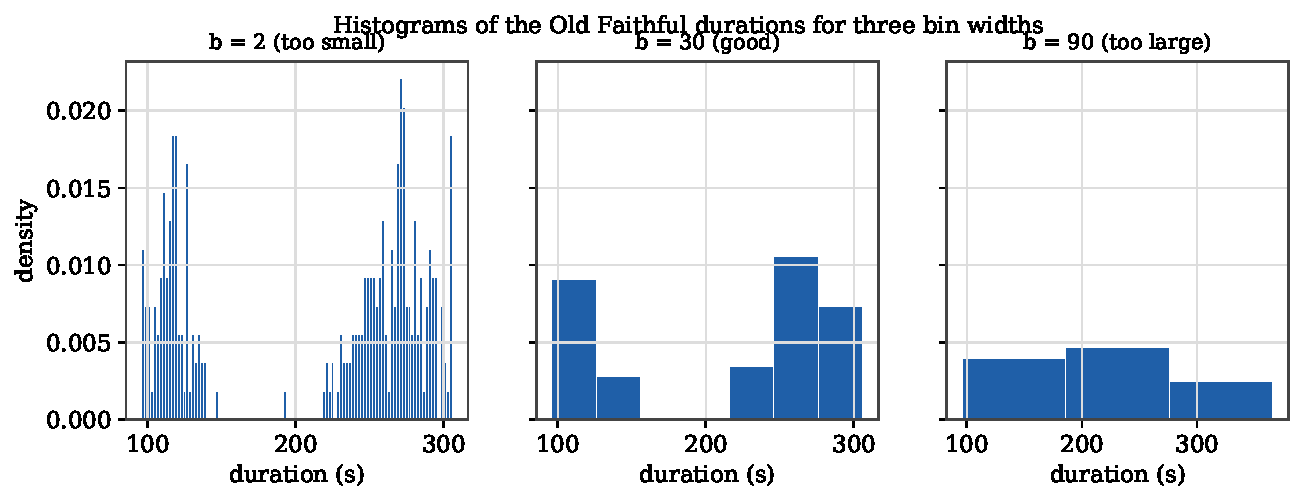
\includegraphics[width=\linewidth]{hist_binwidth}
  \caption{The same geyser data at three bin widths. Too small produces noise;
  too large hides the two modes. In practice one chooses the bin width by trial
  and error until the picture looks reasonable.}
  \label{fig:histbw}
\end{figure}

\subsection{Kernel density estimates}

A histogram is simple but jagged, and sensitive to where the bin edges fall. A
\emph{kernel density estimate} (KDE) produces a smooth curve instead. The idea is
to ``place a small pile of sand'' over each observation and add the piles up;
where data accumulate, the sand piles high. Formally one chooses a \emph{kernel}
$K$—a symmetric density giving each pile its shape—and a \emph{bandwidth} $h$
controlling each pile's width.

\begin{figure}[ht]
  \centering
  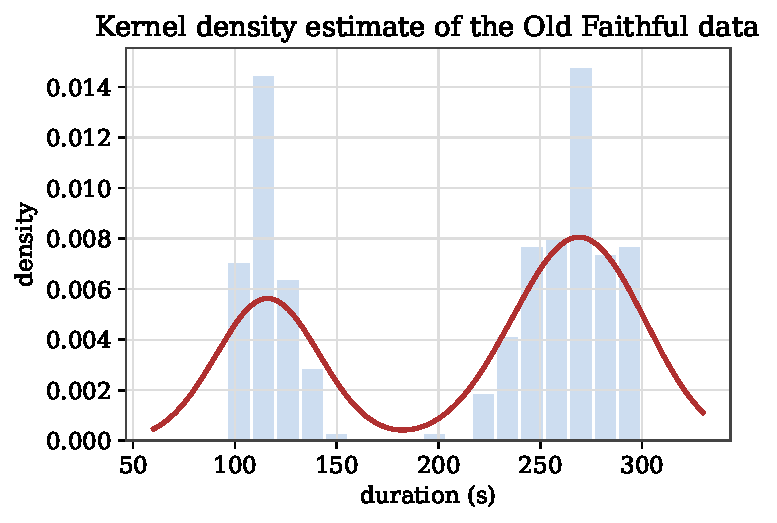
\includegraphics[width=0.62\linewidth]{kde_faithful}
  \caption{A kernel density estimate of the geyser data overlaid on a histogram.
  The two modes are now unmistakable and the curve is smooth.}
  \label{fig:kdefaithful}
\end{figure}

A kernel $K$ typically satisfies $K(u)\ge 0$, integrates to one, is symmetric
about zero, and vanishes outside $[-1,1]$. Common choices include the
Epanechnikov kernel $K(u)=\tfrac34(1-u^2)$ and the triweight kernel
$K(u)=\tfrac{35}{32}(1-u^2)^3$; the normal kernel is also popular, though it
violates the last condition. Figure~\ref{fig:kernels} compares several.

\begin{figure}[ht]
  \centering
  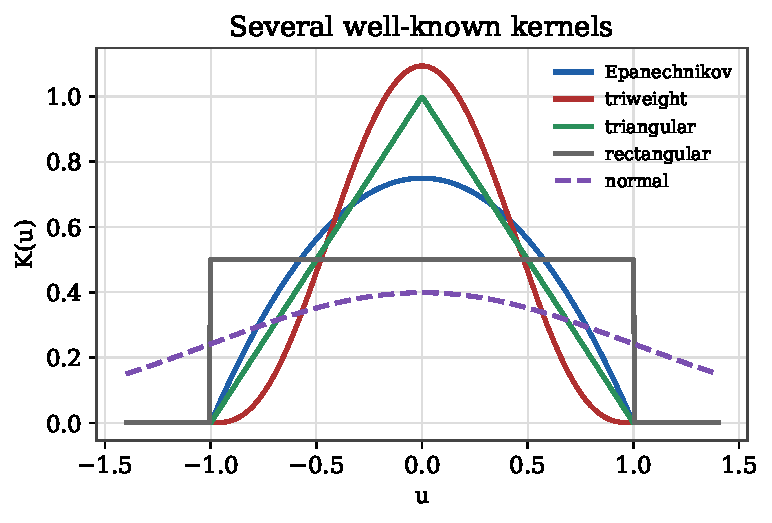
\includegraphics[width=0.6\linewidth]{kernels}
  \caption{Several standard kernels. The choice of kernel matters far less than
  the choice of bandwidth.}
  \label{fig:kernels}
\end{figure}

The bandwidth plays exactly the role the bin width played for the histogram: too
small gives a spiky curve, too large oversmooths and can wash out the modes
(Figure~\ref{fig:kdebw}). The choice of \emph{kernel}, by contrast, has only a
minor effect on the result.

\begin{figure}[ht]
  \centering
  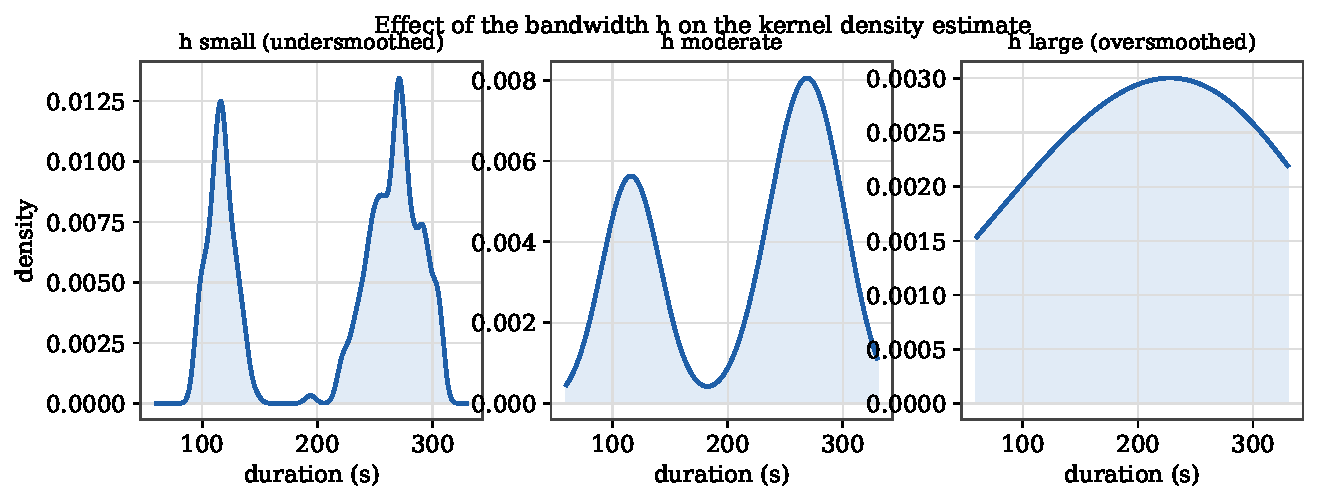
\includegraphics[width=\linewidth]{kde_bandwidth}
  \caption{The bandwidth $h$ controls smoothness. Two well-known kernels with the
  same bandwidth produce nearly identical curves; the bandwidth is what matters.}
  \label{fig:kdebw}
\end{figure}

\subsection{The empirical distribution function}

A third graphical summary plots the data cumulatively. The \emph{empirical
distribution function} (or empirical cdf) is
\[
  F_n(x)=\frac{\text{number of observations}\le x}{n},
\]
the proportion of the dataset at or below $x$. Its graph is a staircase: flat
below the minimum, equal to one above the maximum, and rising by a jump of
$1/n$ at each observation.

\begin{example}[A small empirical cdf]
For the dataset $\{4,3,9,1,7\}$, the empirical cdf is $0$ for $x<1$, jumps to
$\tfrac15$ at $x=1$, to $\tfrac25$ at $x=3$, to $\tfrac35$ at $x=4$, and so on
up to $1$ for $x\ge 9$ (Figure~\ref{fig:ecdftoy}). The closed and open circles
emphasize that the function takes its \emph{higher} value at each jump point.
\end{example}

\begin{figure}[ht]
  \centering
  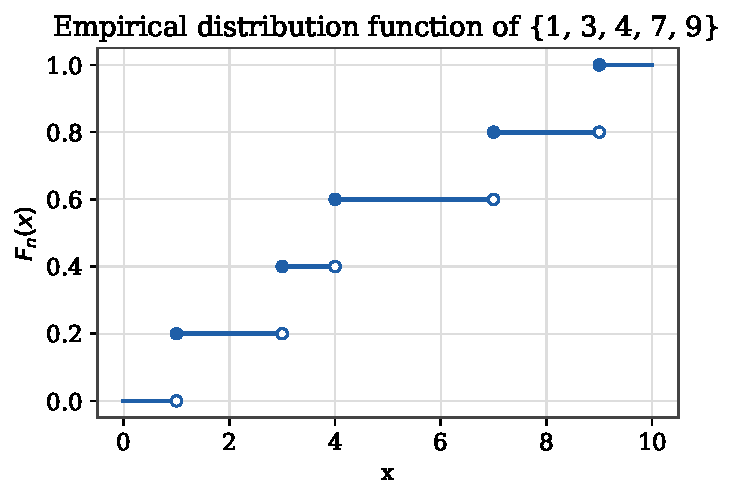
\includegraphics[width=0.52\linewidth]{ecdf_toy}
  \caption{The empirical distribution function of a five-point dataset.}
  \label{fig:ecdftoy}
\end{figure}

For the geyser data (Figure~\ref{fig:ecdffaithful}), the empirical cdf rises
\emph{steeply} where observations crowd together—near $120$ and $270$
seconds—and flattens where they thin out. Steepness of $F_n$ is the cumulative
signature of a mode.

\begin{figure}[ht]
  \centering
  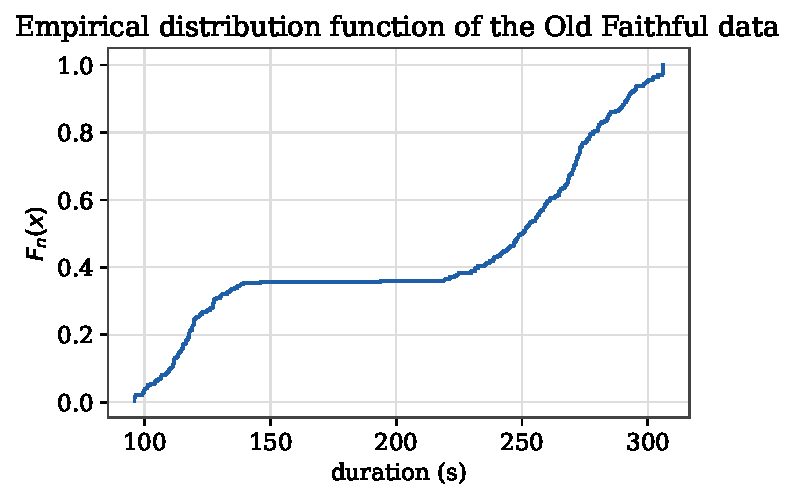
\includegraphics[width=0.52\linewidth]{ecdf_faithful}
  \caption{Empirical distribution function of the geyser data; the two steep
  stretches correspond to the two clusters of durations.}
  \label{fig:ecdffaithful}
\end{figure}

\subsection{The scatterplot}

For a \emph{bivariate} dataset of pairs $(x_1,y_1),\dots,(x_n,y_n)$, the
\emph{scatterplot} simply plots the points. It is the natural first step when we
suspect that $y$ depends on $x$. We will return to scatterplots in
Chapter~\ref{ch:leastsquares}, where we fit lines to them; see, for instance,
the timber and mortality data in that chapter.

\begin{example}[Correlation of geyser eruptions and waiting times]
For the geyser, each eruption's duration can be paired with the waiting time
until the next eruption. The empirical correlation coefficient of these two
quantities is about $0.90$—a strong positive association: long eruptions tend to
be followed by long waits.
\end{example}

\begin{example}[Height and weight, and a prediction]
For a classic dataset of women's heights and weights, fitting a line gives
$\text{height}\approx 0.287\,(\text{weight})+25.72$ inches, with an empirical
correlation of $0.995$—an exceptionally strong linear relationship. Using the
line, a woman weighing $105$ pounds is predicted to be about
$0.287(105)+25.72\approx 56$ inches tall.
\end{example}

\begin{example}[Linearizing exponential growth]
The U.S.\ population appears to grow roughly exponentially, $P(t)=ae^{kt}$.
Taking logarithms turns this into a \emph{linear} relationship,
$\ln P(t)=\ln a + kt$, so regressing $\ln P$ on $t$ recovers the parameters. With
$t$ measured in years from $1790$, this yields $\ln a\approx 1.688$ (so
$a\approx 5.41$ million) and $k\approx 0.0220$, i.e.\ $P(t)\approx 5.41\,e^{0.0220t}$.
Transforming to linearity before fitting is a recurring EDA tactic.
\end{example}

\section{Numerical Summaries}

Graphs reveal shape; numbers pin down location and spread.

\subsection{The center of a dataset}

The \emph{sample mean} is the ordinary average
$\xbar_n=\tfrac1n\sum_{i=1}^n x_i$, the natural analogue of expectation. The
\emph{sample median} is the middle value of the sorted data (the average of the
two middle values when $n$ is even). The mean is sensitive to \emph{outliers};
the median is robust.

\begin{example}[Outliers and a recording error]
Eleven hourly temperatures recorded one New Year's at Wick, Scotland, were
\[
  43,43,41,41,41,42,43,58,58,41,41.
\]
The two $58$'s sit far from the rest and inflate the mean to $44.7$; dropping
them lowers it to $41.8$. The median barely moves ($42$ versus $41$). In fact the
two anomalies arose from a switch of recording units; the corrected values are
near $41$, giving mean $41.5$ and median $42$. The median's robustness is exactly
its insensitivity to such contamination. (This is an argument for being
\emph{aware} of outliers, not for blindly deleting them.)
\end{example}

\subsection{The spread of a dataset}

The \emph{sample variance} and \emph{sample standard deviation} are
\[
  s_n^2=\frac{1}{n-1}\sum_{i=1}^n (x_i-\xbar_n)^2,\qquad s_n=\sqrt{s_n^2}.
\]
The divisor $n-1$ rather than $n$ will be justified in
Chapter~\ref{ch:estimation}, where we show it makes $s_n^2$ unbiased. Like the
mean, the standard deviation is sensitive to outliers: for the uncorrected Wick
data $s_n=6.62$, but only $0.97$ with the two anomalies removed.

A robust alternative is the \emph{median of absolute deviations},
\[
  \MAD(x_1,\dots,x_n)=\Med\bigl(|x_1-\Med_n|,\dots,|x_n-\Med_n|\bigr),
\]
which, like the median, is hardly affected by a few extreme values.

\subsection{Quantiles, quartiles, and the IQR}

The \emph{$p$th empirical quantile} $q_n(p)$ is, loosely, the value below which a
proportion $p$ of the data lie. Writing the sorted data (the \emph{order
statistics}) as $x_{(1)}\le\cdots\le x_{(n)}$, we take the $i$th order statistic
to be the $\tfrac{i}{n+1}$ quantile and interpolate linearly between them.

\begin{example}[Interpolating a percentile]
For the Wick data, the order statistics put $42$ at the $\tfrac{6}{12}=0.5$
quantile and $43$ at the $\tfrac{7}{12}$ quantile. The $55$th percentile lies
between these; linear interpolation between $(0.5,42)$ and $(0.583,43)$ gives
$q_n(0.55)\approx 42.6$.
\end{example}

The lower and upper \emph{quartiles} are $q_n(0.25)$ and $q_n(0.75)$, and the
\emph{interquartile range} is
\[
  \mathrm{IQR}=q_n(0.75)-q_n(0.25),
\]
the span of the middle half of the data—another robust measure of spread.
Together with the minimum, median, and maximum, the quartiles form the
\emph{five-number summary}.

\begin{example}[A five-number summary]
For $1000$ recorded earthquake magnitudes, the five-number summary is
\[
  \min = 4.00,\quad Q_1 = 4.30,\quad \text{median}=4.60,\quad Q_3=4.90,\quad \max=6.40,
\]
with sample mean $4.62$. The closeness of mean and median, and the symmetry of
the quartiles about the median, suggest a roughly symmetric bulk with a modest
right tail.
\end{example}

\subsection{The boxplot}

The \emph{boxplot} renders the five-number summary graphically
(Figure~\ref{fig:boxplot}). A box spans the lower to upper quartile—its height is
the IQR—with a line at the median. \emph{Whiskers} extend to the most extreme
observations within $1.5\times\mathrm{IQR}$ of the box; anything beyond is plotted
individually as a suspected outlier.

\begin{figure}[ht]
  \centering
  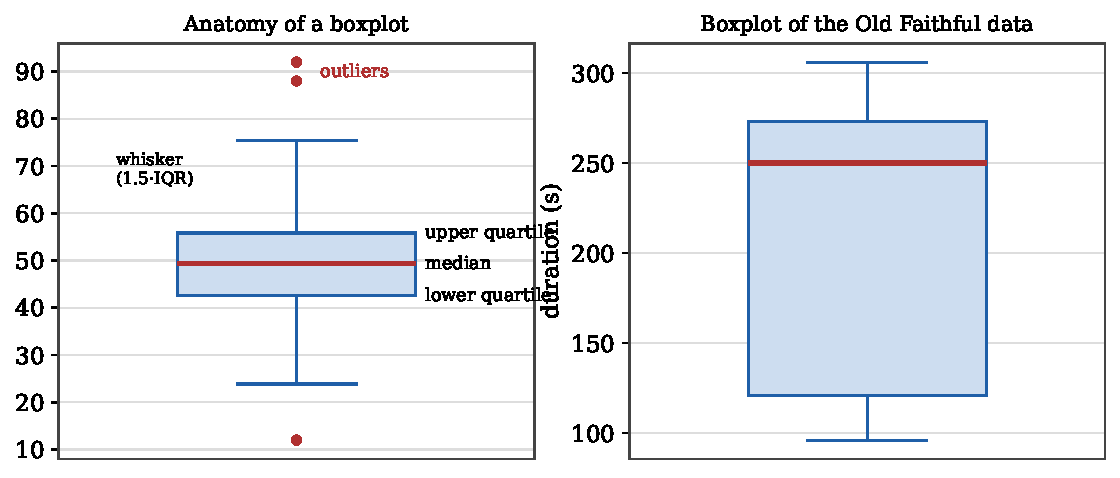
\includegraphics[width=\linewidth]{boxplot}
  \caption{Left: the anatomy of a boxplot. Right: a boxplot of the geyser data.
  Boxplots are excellent for spread and skew but, as here, cannot reveal that a
  dataset is bimodal—the off-center median is the only hint of structure.}
  \label{fig:boxplot}
\end{figure}

The boxplot is superb for comparing spreads and spotting skew and outliers, but
it has a blind spot: it cannot show that the geyser data are \emph{bimodal}. The
position of the median within the box hints at asymmetry, but only the histogram
and KDE reveal the two peaks. No single summary tells the whole story—which is
why exploratory analysis uses several in concert.

\chapter{An Overview of Statistical Inference}
\label{ch:inference}

Exploratory data analysis describes a dataset. \emph{Statistical inference} goes
further: it uses the data to draw conclusions about the unknown distribution that
generated them. Given a sample $X_1,\dots,X_n\sim F$, we want to infer $F$, or
some feature of it such as its mean or variance. This chapter surveys the three
central inference problems—\emph{point estimation}, \emph{confidence intervals},
and \emph{hypothesis testing}—and introduces the $t$ distribution that the later
chapters depend on.

\section{Statistical Models}

A \emph{statistical model} is a set $\mathcal F$ of candidate distributions. A
\emph{parametric} model is one indexed by finitely many parameters, written
$\mathcal F=\{f(x;\theta):\theta\in\Theta\}$, where $\theta$ ranges over a
parameter space $\Theta$. For example, the normal model
\[
  \mathcal F=\Bigl\{\,f(x;\mu,\sigma)=\tfrac{1}{\sigma\sqrt{2\pi}}e^{-\frac12((x-\mu)/\sigma)^2}:\ \mu\in\R,\ \sigma>0\Bigr\}
\]
has two parameters. If only one parameter interests us—say $\mu$—the others are
called \emph{nuisance} parameters. A \emph{nonparametric} model assumes no such
finite-dimensional form; estimating an unknown cdf by the empirical cdf of
Chapter~\ref{ch:eda} is a nonparametric procedure.

\section{Point Estimation}

A \emph{point estimator} of a parameter $\theta$ is a function of the data,
$\hat\theta_n=g(X_1,\dots,X_n)$, intended as a single best guess. Because it
depends on the random sample, $\hat\theta_n$ is itself a random variable, with a
distribution called its \emph{sampling distribution}. Several quantities measure
the quality of an estimator:
\begin{itemize}[leftmargin=1.4em,topsep=2pt,itemsep=1pt]
  \item the \emph{bias}, $\mathrm{bias}(\hat\theta_n)=\E[\hat\theta_n]-\theta$;
        the estimator is \emph{unbiased} if $\E[\hat\theta_n]=\theta$;
  \item the \emph{standard error} $\mathrm{se}=\sqrt{\Var(\hat\theta_n)}$, the
        standard deviation of the sampling distribution (its estimate is
        $\widehat{\mathrm{se}}$);
  \item the \emph{mean squared error}
        $\mathrm{MSE}=\E[(\hat\theta_n-\theta)^2]$.
\end{itemize}
These are linked by a fundamental identity.

\begin{theorem}
The mean squared error decomposes as
$\mathrm{MSE}=\bigl(\mathrm{bias}(\hat\theta_n)\bigr)^2+\Var(\hat\theta_n).$
\end{theorem}

An estimator is \emph{asymptotically normal} if
$(\hat\theta_n-\theta)/\mathrm{se}$ converges to $\N(0,1)$ as $n\to\infty$; many
estimators are, thanks to the central limit theorem.

\begin{example}[Estimating a Bernoulli probability]
Let $X_1,\dots,X_n\sim\Ber(p)$ and let $\hat p_n=\Xbar_n=\tfrac1n\sum X_i$. Then
$\E[\hat p_n]=\tfrac1n\sum\E[X_i]=p$, so $\hat p_n$ is unbiased. Its standard
error is $\mathrm{se}=\sqrt{\Var(\hat p_n)}=\sqrt{p(1-p)/n}$, estimated by
$\widehat{\mathrm{se}}=\sqrt{\hat p_n(1-\hat p_n)/n}$.
\end{example}

\section{Confidence Intervals}

A \emph{$1-\alpha$ confidence interval} for $\theta$ is a random interval
$C_n=(a,b)$, computed from the data, with
\[
  \Prob(\theta\in C_n)\ge 1-\alpha\quad\text{for all }\theta.
\]
We call $1-\alpha$ the \emph{coverage}.

\begin{remark}[How to read a confidence interval]
A confidence interval is \emph{not} a probability statement about $\theta$:
$\theta$ is a fixed (if unknown) number, not random. The randomness is in the
interval. The honest interpretation is a long-run one: if you construct a $95\%$
interval every day—for entirely unrelated parameters—about $95\%$ of those
intervals will trap their target. Each individual interval either contains
$\theta$ or it does not (Figure~\ref{fig:cicov}). When a newspaper reports a poll
``accurate to within $4$ points $95\%$ of the time,'' it is describing exactly
this kind of interval.
\end{remark}

\begin{figure}[ht]
  \centering
  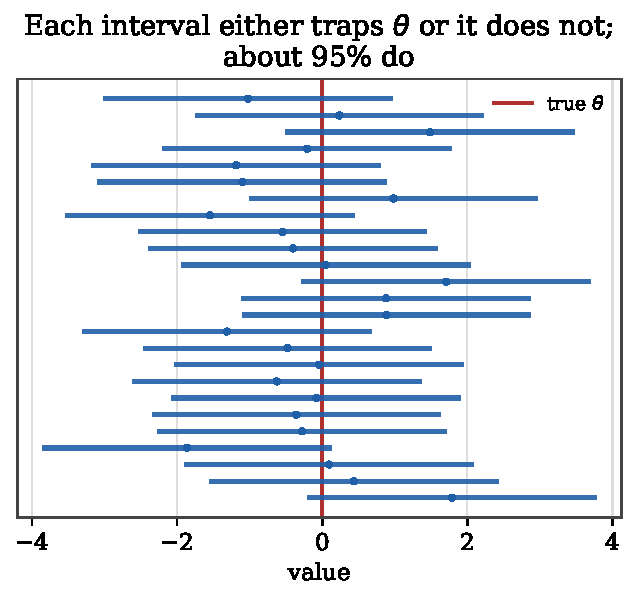
\includegraphics[width=0.5\linewidth]{ci_coverage}
  \caption{Twenty-five $95\%$ confidence intervals for the same $\theta$. About
  one in twenty misses (shown in red). No single interval ``contains $\theta$
  with probability $0.95$''—it either does or does not.}
  \label{fig:cicov}
\end{figure}

\subsection{Normal-based intervals}

When $\hat\theta_n\approx\N(\theta,\widehat{\mathrm{se}}^{\,2})$, we obtain an
approximate interval by going $z_{\alpha/2}$ standard errors either side of the
estimate:
\[
  C_n=\bigl(\hat\theta_n-z_{\alpha/2}\,\widehat{\mathrm{se}},\ \hat\theta_n+z_{\alpha/2}\,\widehat{\mathrm{se}}\bigr),
\]
where $z_{\alpha/2}$ satisfies $\Prob(-z_{\alpha/2}<Z<z_{\alpha/2})=1-\alpha$ for
$Z\sim\N(0,1)$ (Figure~\ref{fig:normalci}). For $95\%$ coverage,
$z_{\alpha/2}=1.96\approx 2$, giving the rule of thumb
$\hat\theta_n\pm 2\,\widehat{\mathrm{se}}$.

\begin{figure}[ht]
  \centering
  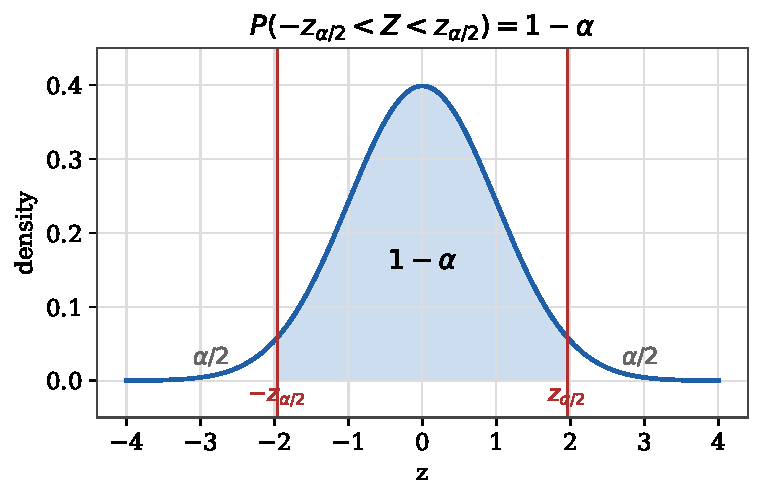
\includegraphics[width=0.55\linewidth]{normal_ci}
  \caption{The critical value $z_{\alpha/2}$ cuts off probability $\alpha/2$ in
  each tail, leaving central probability $1-\alpha$.}
  \label{fig:normalci}
\end{figure}

\begin{example}[Confidence interval for a proportion]
For $X_1,\dots,X_n\sim\Ber(p)$, the CLT gives $\hat p_n\approx\N(p,\mathrm{se}^2)$
for large $n$, so an approximate $1-\alpha$ interval for $p$ is
\[
  \hat p_n\pm z_{\alpha/2}\sqrt{\frac{\hat p_n(1-\hat p_n)}{n}}.
\]
Because we substitute $\widehat{\mathrm{se}}$ for the unknown $\mathrm{se}$, the
coverage is only approximately correct, improving as $n$ grows.
\end{example}

\begin{example}[Known variance: a bottling machine]
A machine fills bottles with volumes that are $\N(\mu,\sigma^2)$ with
$\sigma=5$ ml \emph{known}. A sample of $16$ bottles has $\xbar=743$ ml.
Construct a $95\%$ confidence interval for $\mu$.

\solution With $\sigma$ known, $\Xbar\sim\N(\mu,\sigma^2/n)$ exactly, so
$\mathrm{se}=\sigma/\sqrt n$ and the interval is
\[
  \xbar\pm z_{.025}\frac{\sigma}{\sqrt n}=743\pm 1.96\cdot\frac{5}{\sqrt{16}}=(740.55,\ 745.45)\ \text{ml}. \qedhere
\]
\end{example}

\section{The $t$ Distribution}

In practice $\sigma$ is rarely known and must be estimated from the data by the
sample standard deviation $S_n$. For \emph{small} samples this substitution is
not negligible, and the right reference distribution is no longer the normal but
the $t$ distribution.

\begin{definition}
If $Z\sim\N(0,1)$ and $\chi^2_n$ (a \emph{chi-square} variable with $n$ degrees of
freedom—the sum of squares of $n$ independent standard normals) are independent,
then $T_n=Z/\sqrt{\chi^2_n/n}$ has a \emph{$t$ distribution with $n$ degrees of
freedom}.
\end{definition}

Like the normal, the $t$ density is symmetric about zero, but it has
\emph{thicker tails}, reflecting the extra uncertainty from estimating $\sigma$
(Figure~\ref{fig:ttails}). As the degrees of freedom grow, $\chi^2_n/n\to 1$ by
the law of large numbers, and the $t$ density approaches $\N(0,1)$
(Figure~\ref{fig:tdist}).

\begin{figure}[ht]
  \centering
  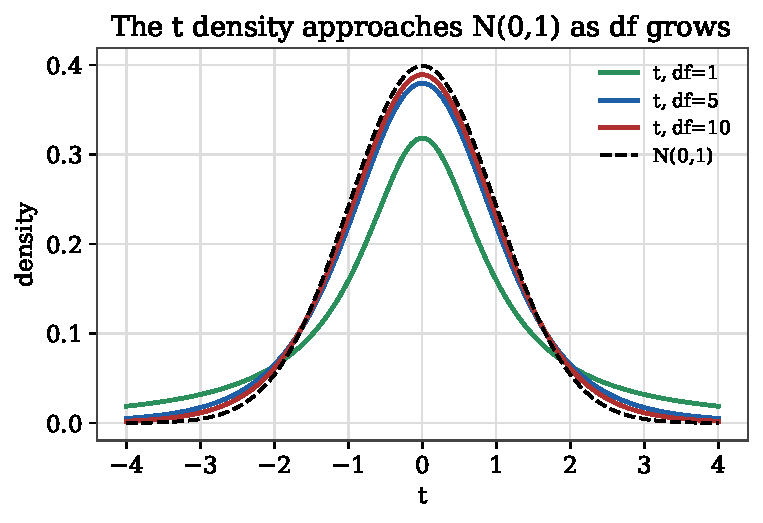
\includegraphics[width=0.6\linewidth]{tdist}
  \caption{The $t$ density with $1$, $5$, and $10$ degrees of freedom, approaching
  $\N(0,1)$ (dashed) as the degrees of freedom increase.}
  \label{fig:tdist}
\end{figure}

\begin{figure}[ht]
  \centering
  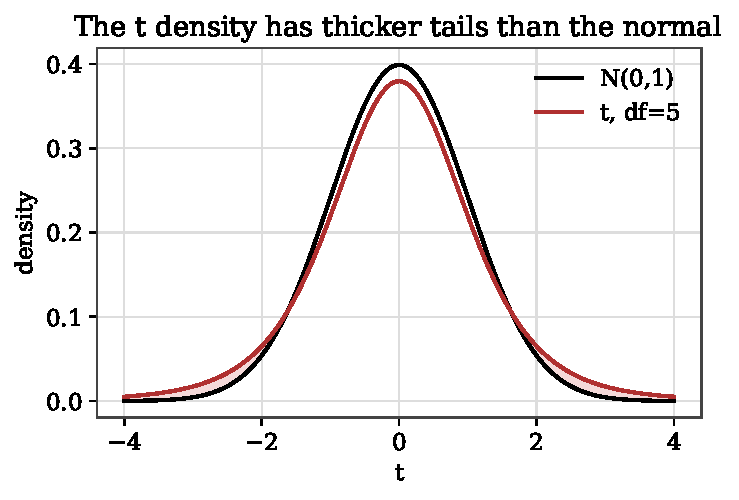
\includegraphics[width=0.5\linewidth]{tdist_tails}
  \caption{The $t$ density (here with $5$ df) has heavier tails than the standard
  normal, accounting for the added variability of an estimated $\sigma$.}
  \label{fig:ttails}
\end{figure}

The key fact is that for an i.i.d.\ $\N(\mu,\sigma^2)$ sample with $\sigma$
unknown,
\[
  \frac{\sqrt n\,(\Xbar_n-\mu)}{S_n}\sim t_{n-1},
\]
\emph{exactly}, not merely approximately. This yields an exact confidence
interval $\xbar\pm t_{\alpha/2,\,n-1}\,s/\sqrt n$ for $\mu$.

\begin{example}[Unknown variance, small sample: caloric content of coal]
Twenty-two measurements of the gross caloric content of a coal shipment give
$\xbar=31.012$ MJ/kg and $s=0.1294$, with the accuracy of the method in doubt
(so $\sigma$ is treated as unknown). Find a $95\%$ confidence interval for the
true mean $\mu$.

\solution With $n=22$ we use $t_{.025,\,21}=2.080$:
\[
  31.012\pm 2.080\cdot\frac{0.1294}{\sqrt{22}}=(30.954,\ 31.069).
\]
This interval is about $50\%$ wider than the corresponding known-$\sigma$
interval would be, both because we use the larger estimate $s$ in place of
$\sigma$ and because the critical value $2.080$ exceeds $1.96$. Estimating the
spread costs us precision.
\end{example}

\begin{example}[Large sample: $t$ and $z$ nearly agree]
A normal sample of size $34$ has $\xbar=3.54$ and $s=0.13$. Construct a $98\%$
confidence interval for $\mu$.

\solution The exact interval uses $t_{.01,\,33}\approx 2.45$:
\[
  3.54\pm 2.45\cdot\frac{0.13}{\sqrt{34}}\approx(3.49,\ 3.59),
\]
while the large-sample approximation with $z_{.01}=2.33$ gives a slightly
narrower $(3.49,3.59)$ as well. For samples this large the $t$ and normal
intervals are nearly identical, which is why the normal approximation is so
widely used.
\end{example}

We summarize the standard intervals.

\begin{center}
\renewcommand{\arraystretch}{1.3}
\begin{tabular}{@{}llll@{}}
\toprule
Situation & Target & Sampling law of $\Xbar$ & $1-\alpha$ interval\\
\midrule
$\Ber(p)$ & $p$ & $\approx$ normal (CLT) & $\xbar\pm z_{\alpha/2}\sqrt{\xbar(1-\xbar)/n}$\\
$\N(\mu,\sigma^2)$, $\sigma$ known & $\mu$ & exactly normal & $\xbar\pm z_{\alpha/2}\,\sigma/\sqrt n$\\
$\N(\mu,\sigma^2)$, $\sigma$ unknown & $\mu$ & $t_{n-1}$ & $\xbar\pm t_{\alpha/2,\,n-1}\,s/\sqrt n$\\
\bottomrule
\end{tabular}
\end{center}

\section{Hypothesis Testing}

The third inference problem starts from a default theory—the \emph{null
hypothesis} $H_0$—and asks whether the data provide enough evidence to reject it
in favor of an \emph{alternative} $H_1$. The logic mirrors a criminal trial: we
presume $H_0$ (innocence) and reject only on strong evidence.

Two errors are possible. A \emph{type I error} rejects a true $H_0$; its
probability is denoted $\alpha$ (the same $\alpha$ as the significance level). A
\emph{type II error} retains $H_0$ when $H_1$ is true; its probability is denoted
$\beta$.

\begin{center}
\renewcommand{\arraystretch}{1.3}
\begin{tabular}{@{}lcc@{}}
\toprule
 & Retain $H_0$ & Reject $H_0$\\
\midrule
$H_0$ true & correct & type I error ($\alpha$)\\
$H_1$ true & type II error ($\beta$) & correct\\
\bottomrule
\end{tabular}
\end{center}

For example, to test whether a coin is fair we would set $H_0:p=\tfrac12$ against
$H_1:p\neq\tfrac12$; to calibrate an automated speed trap so that at most $5\%$ of
ticketed drivers were not actually speeding, we would fix the type I error at
$0.05$. The machinery for carrying out such tests—test statistics, $p$-values,
and significance levels—is developed in Chapters~\ref{ch:leastsquares}
and~\ref{ch:gof}.

\chapter{Point Estimation: Unbiasedness and Efficiency}
\label{ch:estimation}

The previous chapter introduced point estimators and the notions of bias and
variance. This chapter studies them in depth. We first build estimators from data
by matching sample quantities to model quantities, then ask which estimators are
\emph{unbiased}, see how nonlinearity creates bias, and finally compare
unbiased estimators by their variance to find the most \emph{efficient}.

\section{Estimators Built from Data}

A natural way to estimate a parameter is to match a population quantity—a mean, a
probability—to its sample counterpart. The law of large numbers is what makes
this work.

\begin{example}[A binomial parameter from queue data]
At a station, the number of women in each of $100$ queues of length $10$ is
recorded. Modeling the count in a queue as $\Bin(10,p)$, estimate $p$.

\solution If each of the $10$ positions is independently a woman with probability
$p$, the count is $\Bin(10,p)$ with mean $10p$. The sample mean of the counts is
$\xbar=4.35$, which we equate to $10p$, giving $\hat p=0.435$. We matched the
model's mean to the data's mean.
\end{example}

\begin{example}[Two estimators for a geometric parameter]
The number of cycles to pregnancy for $93$ women is recorded, modeled as
$\Geo(p)$. Propose estimators of $p$.

\solution Two natural choices arise. Since $\E[X]=1/p$, we can estimate $\E[X]$
by the sample mean and invert: $\hat p=1/\xbar=93/331$. Alternatively, since
$p=\Prob(X=1)$, we can use the observed fraction of women who conceived in the
first cycle, $\hat p=29/93$. The two estimators—$0.281$ and $0.312$—need not
agree; choosing between them is exactly the kind of question this chapter
addresses. (For the $474$ nonsmoking women, the analogous estimates are
$474/1285=0.369$ and $198/474=0.418$.)
\end{example}

\begin{example}[Was London bombed at random? A Poisson fit]
An area of South London was divided into $576$ quarter-kilometer squares, and the
number of V-bomb hits in each was tallied:
\[
\begin{array}{c|cccccccc}
\text{hits} & 0 & 1 & 2 & 3 & 4 & 5 & 6 & 7\\\hline
\text{squares} & 229 & 211 & 93 & 35 & 7 & 0 & 0 & 1
\end{array}
\]
If hits fall purely at random, the count per square should be Poisson. Estimate
its mean and assess the fit.

\solution Modeling the count as $\Pois(\mu)$ with $\E[X]=\mu$, we estimate $\mu$
by the average number of hits per square,
\[
  \hat\mu=\frac{0\cdot 229+1\cdot 211+2\cdot 93+\cdots+7\cdot 1}{576}\approx 0.93.
\]
Plugging $\hat\mu$ into the Poisson pmf and comparing predicted to observed
relative frequencies:
\[
\begin{array}{c|ccccc}
\text{hits} & 0 & 1 & 2 & 3 & 4\\\hline
\text{observed} & 0.40 & 0.37 & 0.16 & 0.06 & 0.01\\
\text{Poisson} & 0.39 & 0.37 & 0.17 & 0.05 & 0.01
\end{array}
\]
The agreement is remarkable—evidence that the bombing was indeed random rather
than precisely targeted. A formal version of this comparison, the chi-square
goodness-of-fit test, appears in Chapter~\ref{ch:gof}.
\end{example}

\section{Unbiased Estimators}

Recall that $\hat\theta_n$ is \emph{unbiased} for $\theta$ if
$\E[\hat\theta_n]=\theta$. Unbiasedness means the estimator is correct
\emph{on average}, with no systematic over- or under-shooting.

\begin{example}[An unbiased estimator of $\theta^2$]
Let $X_1,\dots,X_n$ be a sample from the uniform distribution on $[-\theta,\theta]$.
Show that $T=\tfrac3n\sum_{i=1}^n X_i^2$ is unbiased for $\theta^2$.

\solution For a $\Unif(-\theta,\theta)$ variable, $\E[X_i]=0$ and
$\Var(X_i)=\tfrac{(2\theta)^2}{12}=\tfrac{\theta^2}{3}$, so
$\E[X_i^2]=\Var(X_i)+\E[X_i]^2=\tfrac{\theta^2}{3}$. By linearity,
\[
  \E[T]=\frac3n\sum_{i=1}^n\E[X_i^2]=\frac3n\cdot n\cdot\frac{\theta^2}{3}=\theta^2. \qedhere
\]
\end{example}

\begin{example}[An unbiased estimator of a probability]
For a $\Geo(p)$ sample, estimate $\Prob(X\le 3)$ by the relative frequency
$S=\tfrac1n\#\{i:X_i\le 3\}$. Show $S$ is unbiased.

\solution Introduce indicators $Y_i=\mathbf 1\{X_i\le 3\}$, so
$\E[Y_i]=\Prob(X_i\le 3)$. Then
\[
  \E[S]=\frac1n\sum_{i=1}^n\E[Y_i]=\Prob(X\le 3).
\]
A relative frequency is always an unbiased estimator of the corresponding
probability—no matter the underlying distribution.
\end{example}

\begin{remark}[Why the sample variance divides by $n-1$]
We can now explain the divisor $n-1$ promised in Chapter~\ref{ch:eda}. For an
i.i.d.\ sample with variance $\sigma^2$, the estimator
$\frac1{n-1}\sum(X_i-\Xbar_n)^2$ is exactly unbiased for $\sigma^2$, whereas
dividing by $n$ would systematically underestimate it (because the deviations are
taken about the sample mean, which is itself pulled toward the data). The
correction factor $\tfrac{n}{n-1}$ removes this downward bias.
\end{remark}

\section{Bias from Nonlinearity}

Unbiasedness is fragile under nonlinear transformation: even if $T$ is unbiased
for $\theta$, $g(T)$ is usually \emph{biased} for $g(\theta)$. Jensen's
inequality (Chapter~\ref{ch:limits}) tells us the \emph{direction} of the bias.

\begin{example}[A square root introduces bias]
With $T=\tfrac3n\sum X_i^2$ unbiased for $\theta^2$ as above, is $\sqrt T$
unbiased for $\theta$?

\solution The function $g(x)=\sqrt x$ is concave, so by Jensen's inequality
$\E[\sqrt T]\le\sqrt{\E[T]}=\sqrt{\theta^2}=\theta$. Thus $\sqrt T$ has
\emph{negative} bias: it tends to underestimate $\theta$.
\end{example}

\begin{example}[Inverting the sample mean]
For a $\Geo(p)$ sample, the law of large numbers suggests $T=1/\Xbar_n$ as an
estimator of $p$ (since $\E[X]=1/p$). Is it unbiased?

\solution The function $g(x)=1/x$ is convex on $(0,\infty)$, so Jensen's
inequality gives $\E[1/\Xbar_n]>1/\E[\Xbar_n]=p$. Hence $T$ has \emph{positive}
bias—it tends to overestimate $p$. Inverting an unbiased estimator does not
preserve unbiasedness.
\end{example}

\begin{example}[An exact bias calculation]
For a $\Pois(\mu)$ sample, the probability of zero arrivals is $e^{-\mu}$, which
one might estimate by $T=e^{-\Xbar_n}$. Compute $\E[T]$.

\solution Write $T=e^{-Z/n}$ with $Z=\sum X_i\sim\Pois(n\mu)$. Then
\[
  \E[T]=\sum_{k=0}^\infty e^{-k/n}\,\frac{(n\mu)^k}{k!}e^{-n\mu}
   =e^{-n\mu}\sum_{k=0}^\infty\frac{(n\mu e^{-1/n})^k}{k!}
   =e^{-n\mu}\,e^{\,n\mu e^{-1/n}}=e^{-n\mu(1-e^{-1/n})}.
\]
Since $1-e^{-1/n}\neq 1/n$, this is not equal to $e^{-\mu}$: the estimator is
biased, though the bias vanishes as $n\to\infty$.
\end{example}

\section{Efficiency: Comparing Unbiased Estimators}

Among unbiased estimators, the better one has the smaller variance (equivalently,
since bias is zero, the smaller MSE). Such an estimator is more \emph{efficient}.

\begin{example}[Optimally combining two sample means]
Two independent samples, of sizes $n$ and $m$ from the same distribution with
mean $\mu$, give sample means $\Xbar_n$ and $\Ybar_m$. Combine them as
$T=r\Xbar_n+(1-r)\Ybar_m$. (a)~Show $T$ is unbiased. (b)~Find the $r$ minimizing
its variance.

\solution (a)~By linearity, $\E[T]=r\mu+(1-r)\mu=\mu$ for every $r$, so $T$ is
unbiased. (b)~By independence,
\[
  \Var(T)=r^2\frac{\sigma^2}{n}+(1-r)^2\frac{\sigma^2}{m}.
\]
Differentiating in $r$ and setting the derivative to zero gives
$\tfrac{2r}{n}-\tfrac{2(1-r)}{m}=0$, i.e.\ $r=\tfrac{n}{n+m}$. The optimal weights
are proportional to the sample sizes—the larger sample is trusted more.
\end{example}

\begin{example}[Pooling two variance estimators]
Independent normal samples of sizes $n$ and $m$ have sample variances $S_X^2$
and $S_Y^2$, both unbiased for the common $\sigma^2$, with
$\Var(S_X^2)=\tfrac{2\sigma^4}{n-1}$ and $\Var(S_Y^2)=\tfrac{2\sigma^4}{m-1}$.
Among estimators $aS_X^2+bS_Y^2$, find the best.

\solution For unbiasedness, $\E[aS_X^2+bS_Y^2]=(a+b)\sigma^2=\sigma^2$ forces
$a+b=1$. Writing $b=1-a$,
\[
  \Var(aS_X^2+(1-a)S_Y^2)=2\sigma^4\Bigl(\frac{a^2}{n-1}+\frac{(1-a)^2}{m-1}\Bigr).
\]
Minimizing over $a$ gives $a=\tfrac{n-1}{n+m-2}$ and hence
$b=\tfrac{m-1}{n+m-2}$. This is the \emph{pooled} variance estimator, weighting
each sample by its degrees of freedom—the standard estimator behind the
two-sample $t$-test.
\end{example}

The maximum likelihood method of the next chapter provides a systematic recipe
for constructing estimators that, under mild conditions, are asymptotically
unbiased and asymptotically the most efficient of all.

\chapter{Maximum Likelihood Estimation}
\label{ch:mle}

The estimators of the previous chapter were built one at a time, by ad hoc
reasoning. We now meet a single, general recipe for producing good
estimators—\emph{maximum likelihood}. The principle is disarmingly simple:
choose the parameter value that makes the observed data most probable.

\section{The Maximum Likelihood Principle}

\begin{principle}[Maximum likelihood]
Given a dataset, estimate the unknown parameter by the value that makes the
observed data as likely as possible.
\end{principle}

A small story fixes the idea. A dealer is offered one of two batches of chips:
one is about $10\%$ defective, the other about $50\%$, but the seller has lost
track of which is which. The dealer tests $10$ chips from a batch and finds
exactly one defective. Which batch is it more likely to be?

\begin{example}[Which batch?]
Test $10$ chips; let $R_i=1$ if chip $i$ is defective. With one defective among
ten, the probability of the observed pattern is $p(1-p)^9$. Compare the two
candidate values of $p$:
\[
  \text{($10\%$ batch)}\ \ (0.1)(0.9)^9\approx 0.039,\qquad
  \text{($50\%$ batch)}\ \ (0.5)(0.5)^9\approx 0.00098.
\]
The observed data are about forty times more likely under the $10\%$ batch, so
the dealer should believe it is that one. This is maximum likelihood reasoning in
miniature.

If instead the \emph{first three} chips were defective, the data probability
becomes $p^3(1-p)^7$, now favoring the $50\%$ batch ($\approx 0.00098$ versus
$\approx 0.00048$): three early defectives are better explained by the
high-defect batch. The data, not a prior hunch, decide.
\end{example}

\begin{example}[Which die?]
A die $D_1$ has five red faces and one white; $D_2$ has one red and five white.
One die is chosen and rolled until red appears, three separate times, giving
first-red on the $3$rd, $5$th, and $4$th rolls. Which die is it likely to be?

\solution The rolls are independent $\Geo(p)$ with $p$ the chance of red, so the
likelihood is
\[
  L(p)=(1-p)^2 p\cdot(1-p)^4 p\cdot(1-p)^3 p=p^3(1-p)^9.
\]
For $D_1$ ($p=\tfrac56$): $L(\tfrac56)\approx 5.74\times10^{-8}$. For $D_2$
($p=\tfrac16$): $L(\tfrac16)\approx 8.97\times10^{-4}$. The data are vastly more
likely under $D_2$, so it is almost surely the mostly-white die.
\end{example}

\section{The Likelihood Function}

For a sample $x_1,\dots,x_n$ from a distribution with parameter $\theta$, the
\emph{likelihood function} is the probability (discrete case) or density
(continuous case) of the data, viewed as a function of $\theta$:
\[
  L(\theta)=\prod_{i=1}^n p_\theta(x_i)\quad\text{(discrete)},\qquad
  L(\theta)=\prod_{i=1}^n f_\theta(x_i)\quad\text{(continuous)}.
\]
The \emph{maximum likelihood estimate} (MLE) is the maximizer
$\hat\theta=\argmax_\theta L(\theta)$.

\begin{example}[The exponential rate]
For a sample from $\Exp(\lambda)$, find the MLE of $\lambda$.

\solution The likelihood is
\[
  L(\lambda)=\prod_{i=1}^n\lambda e^{-\lambda x_i}=\lambda^n e^{-\lambda\sum x_i}.
\]
Differentiating and setting $L'(\lambda)=0$ gives $1-\lambda\xbar_n=0$, so the
MLE is $\hat\lambda=1/\Xbar_n$. (One checks the second derivative is negative
there, confirming a maximum.)
\end{example}

\begin{example}[An endpoint that defies calculus]
A sample $x_1,x_2,x_3=0.98,1.57,0.31$ comes from $\Unif(0,\theta)$ with $\theta$
unknown. Find the MLE of $\theta$.

\solution Each density is $1/\theta$ on $[0,\theta]$ and $0$ outside, so the
likelihood is
\[
  L(\theta)=\begin{cases} 1/\theta^3, & \theta\ge\max(x_i)=1.57,\\ 0, & \theta<1.57.\end{cases}
\]
Differentiating would only show $L$ is decreasing where it is positive; the
maximum sits at the \emph{boundary}. As Figure~\ref{fig:likuniform} shows,
$L(\theta)$ jumps up to its largest value exactly at $\theta=1.57$ and decays
thereafter, so $\hat\theta=\max(x_1,x_2,x_3)=1.57$. In general the MLE for the
upper endpoint is $\max\{X_1,\dots,X_n\}$.
\end{example}

\begin{figure}[ht]
  \centering
  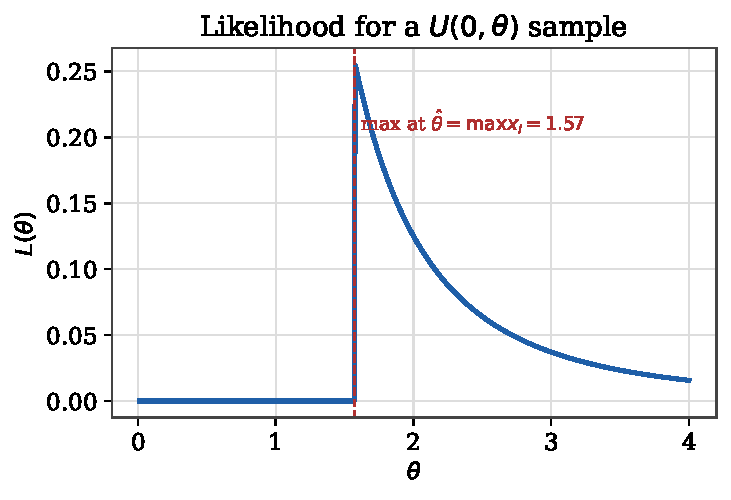
\includegraphics[width=0.5\linewidth]{likelihood_uniform}
  \caption{Likelihood for a $\Unif(0,\theta)$ sample. It is zero until $\theta$
  reaches the largest observation, then decreases—so the maximum is at the
  boundary, where calculus alone would not find it.}
  \label{fig:likuniform}
\end{figure}

\section{The Loglikelihood}

Because $L$ is a product, differentiating it directly means repeated use of the
product rule. Taking logarithms converts the product into a sum, which is far
easier to differentiate; and since the logarithm is increasing, the
\emph{loglikelihood} $\ell(\theta)=\ln L(\theta)$ has its maximum at the same
$\theta$ as $L$.

\begin{example}[Cycles to pregnancy, with censoring]
For $100$ smoking women, the number of cycles to pregnancy is modeled as
$\Geo(p)$; $7$ women had an unknown number exceeding $12$. Counting
$29$ ones, $16$ twos, \dots, and $7$ values above $12$, the likelihood works out
(up to a constant) to
\[
  L(p)=C\,p^{93}(1-p)^{322}.
\]
Find $\hat p$.

\solution The constant $C$ counts arrangements and does not affect the
maximizer. Differentiating,
\[
  L'(p)=C\,p^{92}(1-p)^{321}\bigl(93(1-p)-322p\bigr)=C\,p^{92}(1-p)^{321}(93-415p),
\]
which vanishes (in the interior) at $p=93/415\approx 0.224$. The loglikelihood
$\ell(p)=\ln C+93\ln p+322\ln(1-p)$ has the same maximizer
(Figure~\ref{fig:liksmokers}). Notably $0.224$ is well below the naive estimate
$29/100=0.29$ that ignores the censored women. For the $474$ nonsmokers the
likelihood is $\propto p^{474}(1-p)^{955}$, giving $\hat p=474/1429\approx 0.33$.
\end{example}

\begin{figure}[ht]
  \centering
  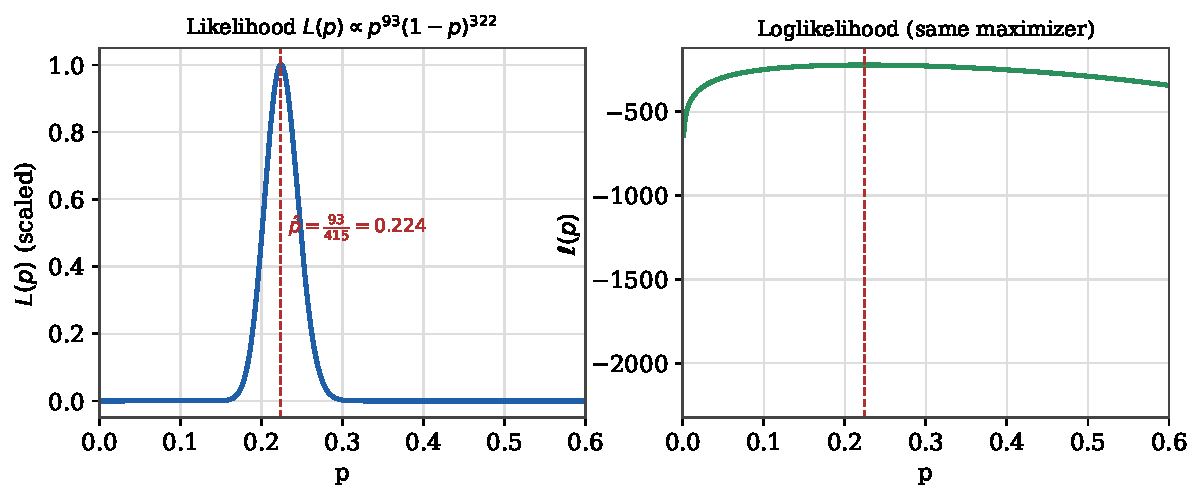
\includegraphics[width=\linewidth]{likelihood_smokers}
  \caption{Likelihood $L(p)\propto p^{93}(1-p)^{322}$ (left) and its
  loglikelihood (right) for the smokers. Both peak at the same value
  $\hat p=93/415\approx 0.224$; the loglikelihood is easier to differentiate.}
  \label{fig:liksmokers}
\end{figure}

\section{The Normal and Poisson MLEs}

\begin{example}[Estimating the mean and standard deviation of a normal]
For an i.i.d.\ $\N(\mu,\sigma^2)$ sample, find the MLEs of $\mu$ and $\sigma$.

\solution The loglikelihood is
\[
  \ell(\mu,\sigma)=-n\ln\sigma-n\ln\sqrt{2\pi}-\frac{1}{2\sigma^2}\sum_{i=1}^n(x_i-\mu)^2.
\]
Setting $\partial\ell/\partial\mu=0$ gives $\hat\mu=\xbar_n$, and then
$\partial\ell/\partial\sigma=0$ gives
\[
  \hat\sigma=\sqrt{\frac1n\sum_{i=1}^n(x_i-\xbar_n)^2}.
\]
(The same two answers follow if one parameter is estimated with the other held
fixed—for instance, with $\mu$ known to be $0$ the MLE of $\sigma$ is
$\sqrt{\tfrac1n\sum x_i^2}$.) Notice the MLE of the variance divides by $n$, not
$n-1$; we return to this below.
\end{example}

\begin{example}[Poisson arrivals, and the probability of none]
Packets arrive at a server, modeled as $\Pois(\mu)$ per minute. (a)~Find the MLE
of $\mu$. (b)~Find the MLE of the probability $e^{-\mu}$ of an idle minute.

\solution (a)~The likelihood is
$L(\mu)=\prod_i \tfrac{\mu^{x_i}}{x_i!}e^{-\mu}=\tfrac{e^{-n\mu}\mu^{\sum x_i}}{\prod x_i!}$,
with loglikelihood $\ell(\mu)=(\sum x_i)\ln\mu - n\mu - \ln\prod x_i!$. Then
$\ell'(\mu)=\tfrac{\sum x_i}{\mu}-n=0$ gives $\hat\mu=\xbar_n$, a maximum since
$\ell''<0$. (Applied to the South London bomb data of
Chapter~\ref{ch:estimation}, this gives $\hat\mu=537/576\approx 0.93$, confirming
the earlier estimate as the MLE.) (b)~By the invariance property below, the MLE
of $e^{-\mu}$ is simply $e^{-\xbar_n}$.
\end{example}

\section{Estimating a Population Size}

\begin{example}[The marked-bolt problem, revisited]
Recall the box of $N$ bolts from Chapter~\ref{ch:discrete}. (a)~If draws
\emph{with} replacement give a $\Geo(1/N)$ sample, find the MLE of $N$. (b)~If
draws \emph{without} replacement give a discrete uniform sample on
$\{1,\dots,N\}$, find the MLE of $N$.

\solution (a)~The loglikelihood for $\Geo(1/N)$ data is
$\ell(N)=-n\ln N+\bigl(\sum x_i-n\bigr)\ln(1-\tfrac1N)$; differentiating and
solving $\ell'(N)=0$ yields, after simplification, $\hat N=\xbar_n$. (b)~For the
discrete uniform, $L(N)=(1/N)^n$ when $N\ge\max x_i$ and $0$ otherwise, a
decreasing function of $N$ on its support. The maximum is again at the boundary:
$\hat N=\max\{X_1,\dots,X_n\}$, the largest value seen—just as for the continuous
uniform endpoint.
\end{example}

\section{Properties of Maximum Likelihood Estimators}

Beyond being a uniform recipe, MLEs enjoy several strong properties.

\paragraph{Invariance.} If $\hat\theta$ is the MLE of $\theta$ and $g$ is an
invertible function, then $g(\hat\theta)$ is the MLE of $g(\theta)$. (This is why
$e^{-\xbar_n}$ is the MLE of $e^{-\mu}$, and why the MLE of $\sigma^2$ is the
square of the MLE of $\sigma$.)

\paragraph{Asymptotic unbiasedness.} An MLE may be biased in finite samples. The
normal-variance MLE $D_n^2=\tfrac1n\sum(X_i-\Xbar_n)^2$ equals
$\tfrac{n-1}{n}S_n^2$, so $\E[D_n^2]=\tfrac{n-1}{n}\sigma^2$—biased downward, but
with the bias vanishing as $n\to\infty$. Under mild conditions every MLE is
asymptotically unbiased: $\lim_{n\to\infty}\E[T_n]=\theta$.

\paragraph{Asymptotic minimum variance.} The variance of any unbiased estimator
is bounded below by the \emph{Cram\'er--Rao} bound, and MLEs attain this bound
asymptotically: no estimator does better in large samples.

\paragraph{Asymptotic normality.} The standardized MLE
$(\hat\theta-\theta)/\widehat{\mathrm{se}}$ converges to $\N(0,1)$. Consequently
\[
  \hat\theta_n\pm 1.96\,\widehat{\mathrm{se}}
\]
is an approximate $95\%$ confidence interval for $\theta$.

\begin{example}[Confidence intervals for the pregnancy parameters]
For the $\Geo(p)$ model, the MLE $\hat p$ has standard error
$\mathrm{se}=\sqrt{p^2(1-p)/n}$. Using asymptotic normality, build approximate
$95\%$ intervals for the smokers ($\hat p=0.224$, $n=100$) and nonsmokers
($\hat p=0.33$, $n=486$).

\solution The interval is $\hat p\pm 1.96\sqrt{\hat p^2(1-\hat p)/n}$. For the
smokers this gives roughly $(0.19,0.26)$, and for the nonsmokers roughly
$(0.31,0.35)$. The two intervals do not overlap, strong evidence that smokers and
nonsmokers really do have different per-cycle conception probabilities.
\end{example}

\chapter{The Method of Least Squares}
\label{ch:leastsquares}

When two quantities are related—a wood's density and its hardness, calcium in
drinking water and a town's mortality—we often want to summarize the relationship
by a line and to use it for prediction. The method of \emph{least squares} fits
such a line by minimizing the total squared vertical distance between the data
and the line. Remarkably, this turns out to be maximum likelihood in disguise,
under the assumption that the measurement errors are normal.

\section{The Simple Linear Regression Model}

The \emph{simple linear regression model} for a bivariate dataset
$(x_1,y_1),\dots,(x_n,y_n)$ treats the $x_i$ as fixed and the responses as random:
\[
  Y_i=\alpha+\beta x_i+U_i,\qquad i=1,\dots,n,
\]
where $U_1,\dots,U_n$ are independent with mean $0$ and variance $\sigma^2$.
Equivalently, $Y_i\sim\N(\alpha+\beta x_i,\sigma^2)$: at each setting of $x$ there
is a whole population of possible responses, normally distributed about the line
$\E[Y]=\alpha+\beta x$, all sharing the same variance. The line's height shifts
with $x$, but the spread does not.

\section{Least Squares Is Maximum Likelihood}

To fit the line we choose $\alpha,\beta$ minimizing the sum of squared vertical
distances
\[
  S(\alpha,\beta)=\sum_{i=1}^n\bigl(y_i-\alpha-\beta x_i\bigr)^2.
\]
This is not an arbitrary choice. Under the normal model the loglikelihood is
\[
  \ell(\alpha,\beta,\sigma)=-n\ln\sigma-n\ln\sqrt{2\pi}-\frac{1}{2\sigma^2}\sum_{i=1}^n(y_i-\alpha-\beta x_i)^2,
\]
which, for any fixed $\sigma$, is maximized precisely when $S(\alpha,\beta)$ is
minimized. Least squares \emph{is} maximum likelihood for normal errors—one
reason normal-error models dominate applications. (Differentiating $\ell$ in
$\sigma$ also gives the MLE
$\hat\sigma=\sqrt{\tfrac1n\sum(Y_i-\hat\alpha-\hat\beta x_i)^2}$.)

As Figure~\ref{fig:ssparab} suggests, $S(\alpha,\beta)$ is an upward-opening
bowl (an elliptic paraboloid), so it has a unique minimum—except in the
degenerate case where all $x_i$ are equal.

\begin{figure}[ht]
  \centering
  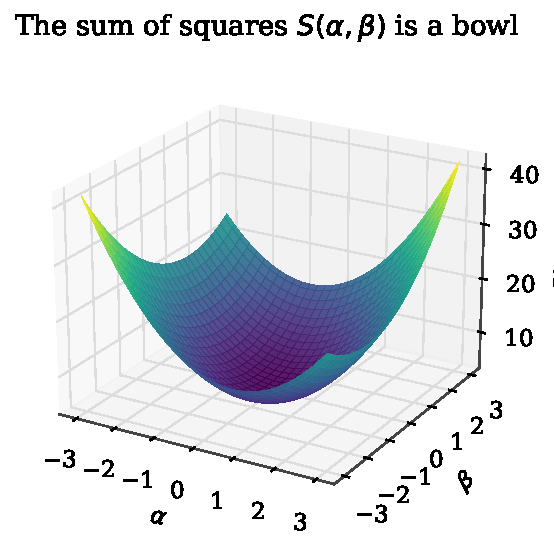
\includegraphics[width=0.52\linewidth]{ss_paraboloid}
  \caption{The sum-of-squares surface $S(\alpha,\beta)$ is a bowl with a single
  lowest point $(\hat\alpha,\hat\beta)$.}
  \label{fig:ssparab}
\end{figure}

\section{The Normal Equations and the Estimates}

Setting the partial derivatives of $S$ to zero yields the \emph{normal
equations}
\[
  n\alpha+\beta\sum x_i=\sum y_i,\qquad
  \alpha\sum x_i+\beta\sum x_i^2=\sum x_iy_i,
\]
a $2\times 2$ linear system whose solution is the pair of least-squares estimates
\[
  \hat\beta=\frac{n\sum x_iy_i-(\sum x_i)(\sum y_i)}{n\sum x_i^2-(\sum x_i)^2},
  \qquad \hat\alpha=\ybar_n-\hat\beta\,\xbar_n.
\]
The second formula shows that the fitted line always passes through the center of
mass $(\xbar_n,\ybar_n)$ of the data.

\begin{example}[A three-point fit]
Fit the least-squares line to $(1,2),(3,1.8),(5,1)$, and find the residuals.

\solution With $\sum x_i=9$, $\sum y_i=4.8$, $\sum x_i^2=35$, $\sum x_iy_i=12.4$,
and $n=3$,
\[
  \hat\beta=\frac{3(12.4)-9(4.8)}{3(35)-9^2}=-0.25,\qquad
  \hat\alpha=1.6-(-0.25)(3)=2.35,
\]
so the line is $y=2.35-0.25x$ (Figure~\ref{fig:toyreg}). The residuals
$r_i=y_i-\hat\alpha-\hat\beta x_i$ are $-0.1,\,0.2,\,-0.1$, which sum to zero—as
they always must.
\end{example}

\begin{figure}[ht]
  \centering
  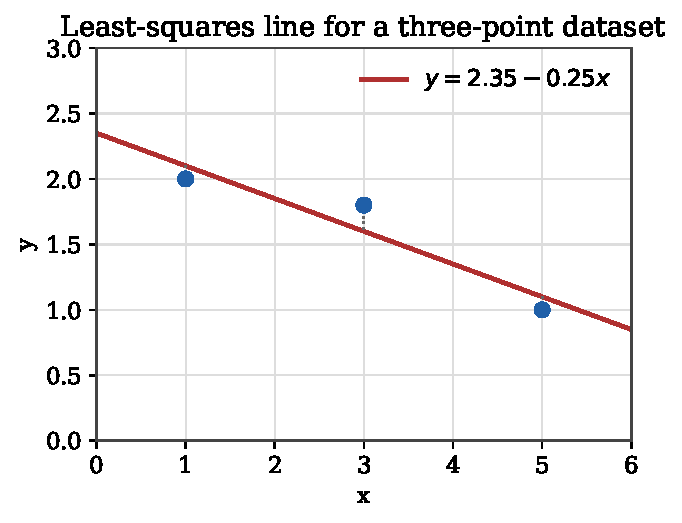
\includegraphics[width=0.42\linewidth]{toy_regression}
  \caption{The least-squares line for three points; the dotted segments are the
  residuals being minimized.}
  \label{fig:toyreg}
\end{figure}

\begin{example}[Predicting timber hardness]
For $36$ Australian hardwoods, regressing Janka hardness on density gives
$\hat\alpha=-1160.5$ and $\hat\beta=57.51$. Predict the hardness of a specimen of
density $65$.

\solution Substitute into the fitted line:
$\hat y=-1160.5+57.51(65)\approx 2577.7$. The regression line turns an
easily-measured density into a prediction of the hard-to-measure hardness.
\end{example}

\section{Unbiasedness of the Estimators}

The least-squares estimators are unbiased.

\begin{example}[$\hat\beta$ is unbiased]
Show $\E[\hat\beta]=\beta$ in the model $Y_i=\alpha+\beta x_i+U_i$.

\solution Since the $x_i$ are constants and $\E[Y_i]=\alpha+\beta x_i$, linearity
gives
\[
  \E[\hat\beta]=\frac{n\sum x_i\E[Y_i]-(\sum x_i)(\sum\E[Y_i])}{n\sum x_i^2-(\sum x_i)^2}
   =\frac{n\sum x_i(\alpha+\beta x_i)-(\sum x_i)\sum(\alpha+\beta x_i)}{n\sum x_i^2-(\sum x_i)^2}.
\]
The $\alpha$-terms cancel and the numerator collapses to
$\beta\bigl(n\sum x_i^2-(\sum x_i)^2\bigr)$, which is exactly the denominator
times $\beta$. Hence $\E[\hat\beta]=\beta$. It follows that
$\E[\hat\alpha]=\E[\Ybar_n]-\xbar_n\E[\hat\beta]=(\alpha+\beta\xbar_n)-\xbar_n\beta=\alpha$,
so $\hat\alpha$ is unbiased too.
\end{example}

For the error variance, the MLE $\tfrac1n\sum(Y_i-\hat\alpha-\hat\beta x_i)^2$
turns out to have expectation $\tfrac{n-2}{n}\sigma^2$, so the \emph{unbiased}
estimator divides by $n-2$ instead:
\[
  \hat\sigma^2=\frac{1}{n-2}\sum_{i=1}^n\bigl(Y_i-\hat\alpha-\hat\beta x_i\bigr)^2.
\]
We lose two degrees of freedom because two parameters, $\alpha$ and $\beta$, were
estimated from the same data.

\section{Residuals and Model Checking}

The \emph{residuals} $r_i=y_i-\hat\alpha-\hat\beta x_i$ are the leftover vertical
distances. They always sum to zero (because the line passes through
$(\xbar,\ybar)$), and plotting them against $x_i$ is the standard diagnostic. If
the linear model is right, the residual plot should look like featureless random
scatter about zero, as for the black cherry tree data
(Figure~\ref{fig:resgood}).

\begin{figure}[ht]
  \centering
  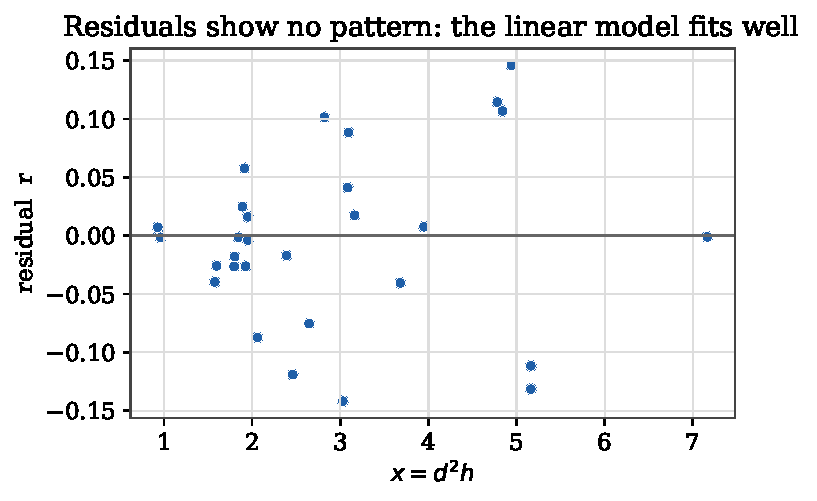
\includegraphics[width=0.55\linewidth]{residuals_good}
  \caption{Residuals with no trend: the linear model is adequate.}
  \label{fig:resgood}
\end{figure}

A \emph{pattern} in the residuals signals a misspecified model. For the timber
data, the residuals from a straight-line fit bend in a parabola
(Figure~\ref{fig:restimber}, left), suggesting a quadratic term:
\[
  Y_i=\alpha+\beta x_i+\gamma x_i^2+U_i.
\]
(This is still called a \emph{linear} model—linear in the parameters
$\alpha,\beta,\gamma$, even though the fitted curve is a parabola; see
Figure~\ref{fig:timberscatter}.) After adding the quadratic term, the residuals
lose their bend but begin to \emph{fan out} (Figure~\ref{fig:restimber}, right):
their spread grows with $x$. This is \emph{heteroscedasticity}—a violation of the
equal-variance assumption—as opposed to the constant-variance ideal of
\emph{homoscedasticity}. One remedy is weighted least squares, which we do not
pursue here.

\begin{figure}[ht]
  \centering
  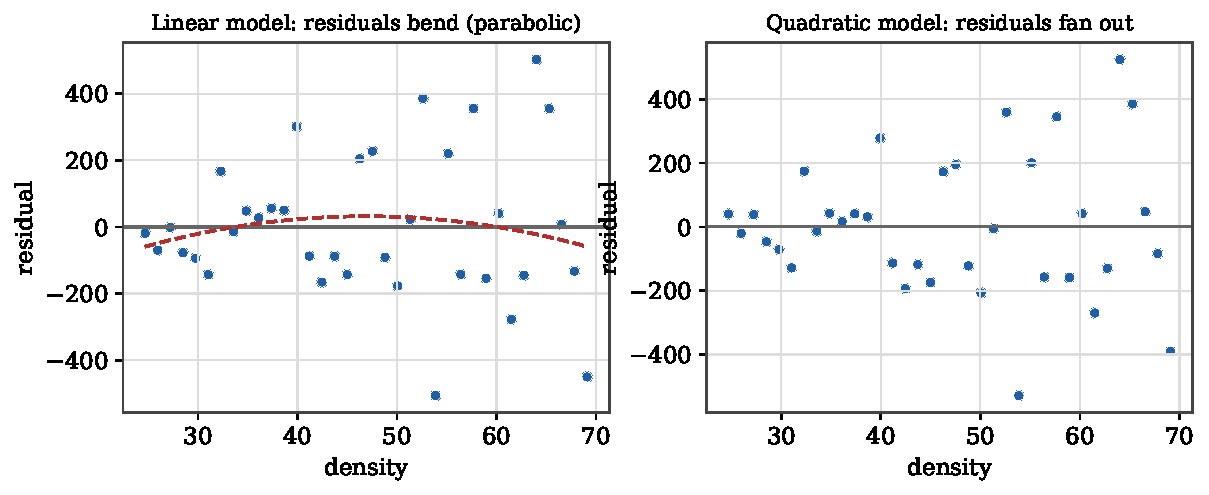
\includegraphics[width=\linewidth]{residuals_timber}
  \caption{Left: a straight-line fit to the timber data leaves a parabolic
  trend. Right: after adding a quadratic term the trend is gone, but the
  residuals fan out, revealing heteroscedasticity.}
  \label{fig:restimber}
\end{figure}

\begin{figure}[ht]
  \centering
  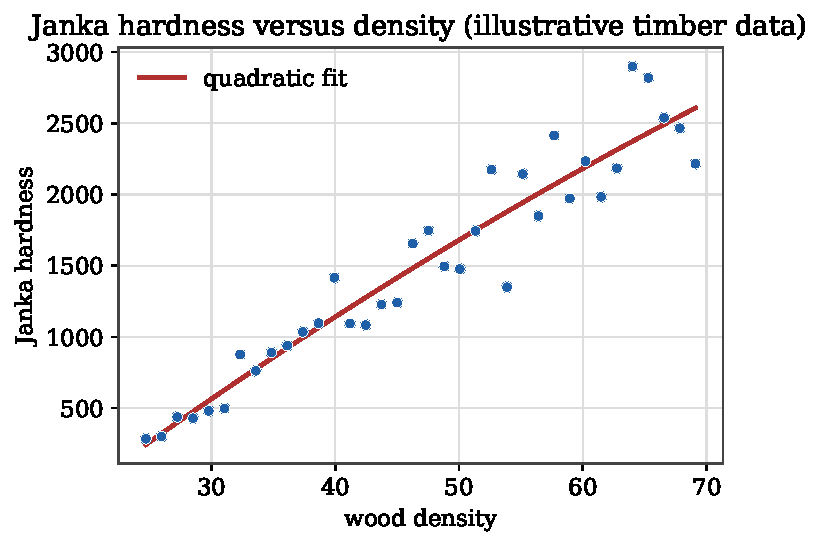
\includegraphics[width=0.5\linewidth]{timber_scatter}
  \caption{Janka hardness versus density with a fitted quadratic. The model is
  linear in its parameters even though the curve is not a straight line.}
  \label{fig:timberscatter}
\end{figure}

\section{Regression Through the Origin}

Sometimes the intercept should be zero on physical grounds. For the black cherry
tree data, the response $y$ is timber volume and the predictor is $x=d^2h$
(diameter squared times height); as a tree shrinks to nothing, $x\to 0$ forces
$y\to 0$, so the model $Y_i=\beta x_i+U_i$ with no intercept is natural.

\begin{example}[The no-intercept slope]
Minimize $S(\beta)=\sum(y_i-\beta x_i)^2$ to derive the slope estimate.

\solution Differentiating, $S'(\beta)=-2\sum(y_i-\beta x_i)x_i=0$ gives
\[
  \hat\beta=\frac{\sum_{i=1}^n x_iy_i}{\sum_{i=1}^n x_i^2}. \qedhere
\]
\end{example}

\begin{example}[Three competing slope estimators]
For the no-intercept model, three natural estimators of $\beta$ are the average of
ratios $B_1=\tfrac1n\sum\tfrac{Y_i}{x_i}$, the ratio of averages
$B_2=\tfrac{\sum Y_i}{\sum x_i}$, and the least-squares estimator
$B_3=\tfrac{\sum x_iY_i}{\sum x_i^2}$. Show all three are unbiased, and compare
them on the cherry tree data.

\solution Each is a linear combination of the $Y_i$ with $\E[Y_i]=\beta x_i$, so
$\E[B_1]=\E[B_2]=\E[B_3]=\beta$: all unbiased. Numerically, using
$\sum x_i=87.456$, $\sum y_i=26.486$, $\sum y_i/x_i=9.369$, $\sum x_iy_i=95.498$,
$\sum x_i^2=314.644$, the three estimates are
\[
  B_1\approx 0.302,\qquad B_2\approx 0.303,\qquad B_3\approx 0.3035.
\]
They are close but not identical (Figure~\ref{fig:cherryreg}). Unbiasedness alone
does not single out a winner—efficiency does, and the least-squares estimator
$B_3$ is the one with smallest variance.
\end{example}

\begin{figure}[ht]
  \centering
  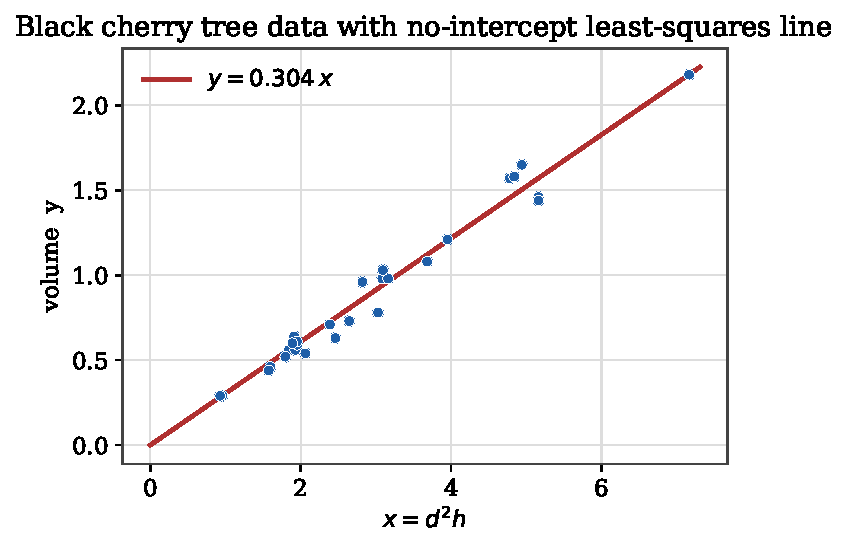
\includegraphics[width=0.5\linewidth]{cherry_regression}
  \caption{Black cherry tree volumes against $x=d^2h$ with the no-intercept
  least-squares line.}
  \label{fig:cherryreg}
\end{figure}

\section{Testing Whether a Coefficient Belongs}

A central question in regression is whether a coefficient is really nonzero, or
whether the apparent effect could be chance. We test, say, $H_0:\beta=\beta_0$
using a \emph{test statistic}
\[
  T_b=\frac{\hat\beta-\beta_0}{S_b},\qquad S_b^2=\frac{n}{n\sum x_i^2-(\sum x_i)^2}\,\hat\sigma^2,
\]
which standardizes the estimate by an estimate of its standard deviation. Under
$H_0$, $T_b$ has a $t$ distribution with $n-2$ degrees of freedom. Values near
zero support $H_0$; large values argue against it.

The strength of evidence is summarized by a \emph{$p$-value}—the probability,
\emph{if $H_0$ were true}, of a test statistic at least as extreme as the one
observed. A small $p$-value is strong evidence against $H_0$. If we reject when
the $p$-value falls below a threshold, that threshold is the \emph{significance
level}. A common informal scale:
\begin{center}
\renewcommand{\arraystretch}{1.15}
\begin{tabular}{@{}ll@{}}
\toprule
$p$-value & evidence against $H_0$\\
\midrule
$<0.01$ & very strong\\
$0.01$--$0.05$ & strong\\
$0.05$--$0.10$ & weak\\
$>0.10$ & little to none\\
\bottomrule
\end{tabular}
\end{center}

\begin{remark}
The $p$-value is \emph{not} $\Prob(H_0\text{ true}\mid\text{data})$—that
quantity belongs to Bayesian inference. The $p$-value is the smallest
significance level at which the data would lead us to reject $H_0$.
\end{remark}

\begin{example}[Does the cherry-tree intercept belong?]
Fitting the cherry tree data \emph{with} an intercept and testing $H_0:\alpha=0$
(we expect no intercept, since zero size should mean zero volume), the test
statistic is $t_a=-0.428$ on $29$ degrees of freedom, giving a one-sided
$p$-value $\Prob(t_{29}\le -0.428)=0.336$.

\solution This $p$-value is large, so we retain $H_0$: the data are entirely
consistent with a zero intercept, confirming the physical reasoning behind the
no-intercept model.
\end{example}

\begin{example}[Does calcium affect mortality?]
For $61$ English towns, mortality rate $y$ is regressed on calcium concentration
$x$ (Figure~\ref{fig:mortality}). We test $H_0:\beta=0$ against $H_1:\beta<0$
(more calcium, lower mortality). The fit gives $\hat\beta=-3.226$ and
$s_b=0.485$, so $t_b=-6.656$ on $59$ degrees of freedom.

\solution The corresponding $p$-value is about $5\times10^{-9}$—overwhelming
evidence against $H_0$. We conclude that higher calcium concentrations are
genuinely associated with lower mortality, not an artifact of chance.
\end{example}

\begin{figure}[ht]
  \centering
  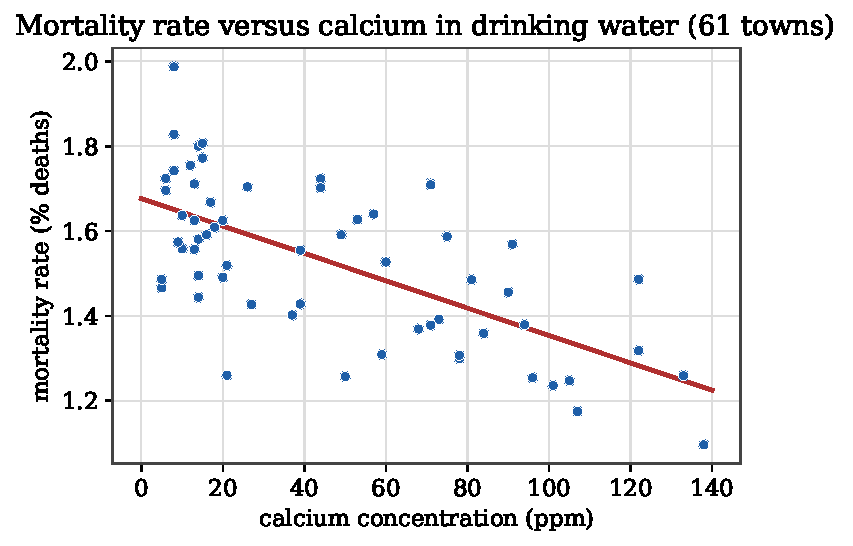
\includegraphics[width=0.52\linewidth]{mortality_scatter}
  \caption{Mortality rate against calcium concentration for $61$ towns, with the
  least-squares line. The downward slope is highly significant.}
  \label{fig:mortality}
\end{figure}

\section{Reading a Regression Summary}

Statistical software reports several diagnostics for a fitted regression. The most
important is $R^2$, the \emph{coefficient of determination},
\[
  R^2=1-\frac{SS_{\mathrm{res}}}{SS_{\mathrm{tot}}},\qquad
  SS_{\mathrm{res}}=\sum_i(y_i-\hat y_i)^2,\quad SS_{\mathrm{tot}}=\sum_i(y_i-\ybar)^2,
\]
the fraction of the response's variation explained by the model. In simple linear
regression $R^2$ is just the square of the empirical correlation coefficient.
Figure~\ref{fig:rsq} illustrates the idea: $SS_{\mathrm{tot}}$ measures spread
about the flat mean line, $SS_{\mathrm{res}}$ about the fitted line; the more the
line shrinks the squares, the closer $R^2$ is to one.

\begin{figure}[ht]
  \centering
  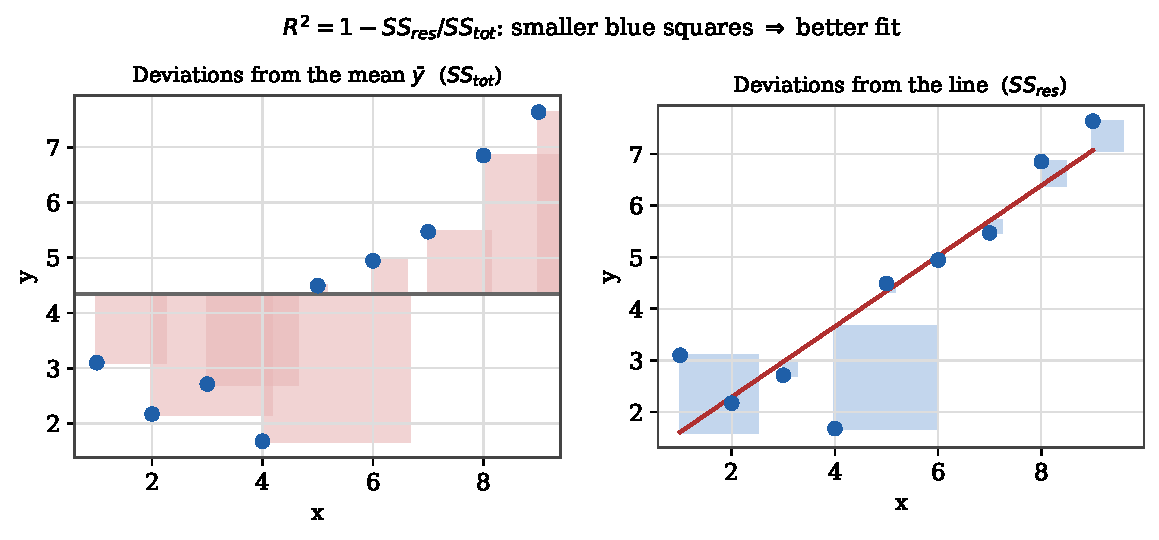
\includegraphics[width=\linewidth]{r_squared}
  \caption{$R^2=1-SS_{\mathrm{res}}/SS_{\mathrm{tot}}$. The red squares (left)
  measure deviations from the mean; the blue squares (right) measure deviations
  from the fitted line. Smaller blue squares mean a better fit and larger $R^2$.}
  \label{fig:rsq}
\end{figure}

A summary also reports the \emph{adjusted} $R^2$, which penalizes extra
parameters and so guards against overfitting; the \emph{residual standard error},
$\hat\sigma$ on $n-2$ degrees of freedom (two parameters estimated); and an
\emph{$F$-test} of whether the regression coefficients are jointly zero. In
simple linear regression the $F$-test merely echoes the $t$-test for the slope,
but it becomes genuinely informative when several predictors are present.

Finally, $95\%$ confidence intervals for the parameters are obtained from the $t$
distribution with $n-2$ degrees of freedom. For the mortality data, the interval
for the calcium slope $\beta$ is about $(-0.0042,-0.0023)$—comfortably below
zero, consistent with the highly significant test above. For the quadratic timber
fit, the intercept's interval $(-804,556)$ comfortably contains zero, as physical
reasoning predicts, while the quadratic coefficient's interval
$(0.19,0.82)$ excludes zero, confirming that the curvature is real. Wide
intervals like the timber ones can be narrowed only by gathering more data.

\chapter{Testing for Goodness of Fit}
\label{ch:gof}

We close with a question that has run quietly beneath the whole second half of
the book: does a proposed probability model actually \emph{fit} the data? When we
modeled bomb hits as Poisson or pea types by Mendel's ratios, we compared
observed and predicted frequencies informally. This chapter makes the comparison
rigorous through the likelihood ratio test and Pearson's chi-square test.

\section{Is There a ``Best'' Test?}

First, some vocabulary. A hypothesis fixing a parameter exactly, like
$\theta=\theta_0$, is \emph{simple}; one allowing a range, like $\theta>\theta_0$,
is \emph{composite}. A test of $H_0:\theta=\theta_0$ against $H_1:\theta\neq\theta_0$
is \emph{two-sided}; a test against $H_1:\theta>\theta_0$ is \emph{one-sided}.
Recall the two error probabilities, $\alpha$ (type I) and $\beta$ (type II); the
\emph{power} of a test is $1-\beta$, its chance of correctly rejecting a false
$H_0$. The usual strategy fixes $\alpha$ and seeks the largest possible power. A
test achieving the most power among all level-$\alpha$ tests is \emph{most
powerful}.

Most powerful tests are hard to find and often do not exist. But in the simplest
case they do, and they take a memorable form.

\begin{theorem}[Neyman--Pearson lemma]
To test the simple $H_0:\theta=\theta_0$ against the simple $H_1:\theta=\theta_1$,
form the likelihood ratio
\[
  T=\frac{L(\theta_1)}{L(\theta_0)}=\frac{\prod_i f(x_i;\theta_1)}{\prod_i f(x_i;\theta_0)},
\]
and reject $H_0$ when $T>k$. Choosing $k$ so that $\Prob_{\theta_0}(T>k)=\alpha$
yields the most powerful level-$\alpha$ test.
\end{theorem}

In words: when both hypotheses are simple and there are no nuisance parameters,
the optimal test compares how well the two parameter values explain the data,
through a ratio of likelihoods.

\section{The Likelihood Ratio Test}

Real problems usually involve composite hypotheses or nuisance parameters, where
the Neyman--Pearson lemma does not directly apply. The \emph{likelihood ratio
test} generalizes its idea. To test $H_0:\theta\in\Theta_0$ against
$H_1:\theta\notin\Theta_0$, the test statistic is
\[
  \lambda=2\ln\!\left(\frac{\max_{\theta\in\Theta}L(\theta)}{\max_{\theta\in\Theta_0}L(\theta)}\right)
   =2\ln\!\left(\frac{L(\hat\theta)}{L(\hat\theta_0)}\right),
\]
the (twice log) ratio of the best fit overall to the best fit allowed under
$H_0$. Large $\lambda$ means $H_0$ explains the data far worse than the
unrestricted model, and counts against $H_0$. Its calibration is a theorem.

\begin{theorem}
Under $H_0$, as $n\to\infty$ the statistic $\lambda$ converges to a chi-square
distribution whose degrees of freedom equal the difference in dimension between
$\Theta$ and $\Theta_0$. The $p$-value is the upper-tail probability
$\Prob(\chi^2_{r-q}>\lambda)$.
\end{theorem}

The chi-square family (Figure~\ref{fig:chisq}) thus governs goodness-of-fit
testing, just as the normal and $t$ families governed estimation.

\begin{figure}[ht]
  \centering
  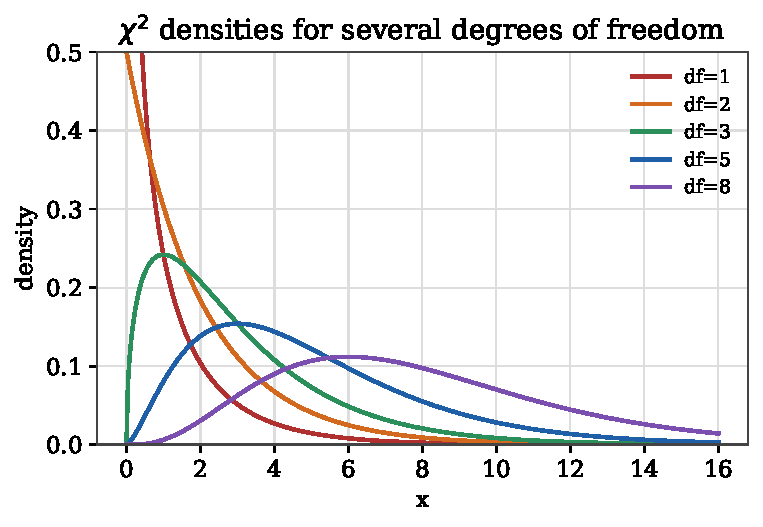
\includegraphics[width=0.55\linewidth]{chisq}
  \caption{Chi-square densities. The degrees of freedom—the difference in
  dimension between the full and restricted parameter spaces—determine which
  curve calibrates the test.}
  \label{fig:chisq}
\end{figure}

\section{The Multinomial Distribution}

Goodness-of-fit data are counts in categories, which follow a \emph{multinomial}
distribution—the multivariate cousin of the binomial. Drawing $n$ times
independently from $k$ categories with probabilities $p=(p_1,\dots,p_k)$, and
letting $X_j$ count category $j$, gives $X\sim\Mult(n,p)$ with
\[
  \Prob(X=x)=\binom{n}{x_1\cdots x_k}p_1^{x_1}\cdots p_k^{x_k}.
\]
Each $X_j$ is marginally $\Bin(n,p_j)$, so $\E[X_j]=np_j$.

\begin{example}[The multinomial MLE]
Show that the MLE of $p$ for multinomial data is $\hat p_j=X_j/n$.

\solution Ignoring a constant, the loglikelihood is
$\ell(p)=\sum_j X_j\ln p_j$, to be maximized subject to $\sum_j p_j=1$. Using a
Lagrange multiplier $\lambda$, maximize
$\sum_j X_j\ln p_j+\lambda(\sum_j p_j-1)$. Setting
$\partial/\partial p_j=\tfrac{X_j}{p_j}+\lambda=0$ gives $\hat p_j=-X_j/\lambda$,
and the constraint $\sum_j\hat p_j=1$ forces $\lambda=-n$, so
$\hat p_j=X_j/n$—each category's observed proportion.
\end{example}

\section{Pearson's Chi-Square Test}

To test a fully specified $H_0:p=p_0$ against $H_1:p\neq p_0$, Pearson's
chi-square statistic compares observed counts $X_j$ to the counts $E_j=np_j$
expected under $H_0$:
\[
  T=\sum_{j=1}^k\frac{(X_j-E_j)^2}{E_j}.
\]
Under $H_0$, $T$ converges to $\chi^2_{k-1}$ (one degree of freedom is lost to the
constraint $\sum X_j=n$), and the $p$-value is $\Prob(\chi^2_{k-1}>t)$. Pearson's
statistic is in fact a second-order Taylor approximation to the likelihood ratio
statistic $\lambda$—a computational shortcut from $1900$, when logarithms were
laborious—so the two give nearly identical answers.

\begin{example}[Mendel's peas]
Mendel's theory predicts that round-yellow, wrinkled-yellow, round-green, and
wrinkled-green peas occur in proportions
$p_0=(\tfrac{9}{16},\tfrac{3}{16},\tfrac{3}{16},\tfrac{1}{16})$. In $n=556$ plants
he observed $X=(315,101,108,32)$. Test $H_0:p=p_0$.

\solution The expected counts are $np_0=(312.75,104.25,104.25,34.75)$
(Figure~\ref{fig:mendel}). Pearson's statistic is
\[
  t=\frac{(315-312.75)^2}{312.75}+\frac{(101-104.25)^2}{104.25}+\frac{(108-104.25)^2}{104.25}+\frac{(32-34.75)^2}{34.75}=0.47.
\]
With $k=4$ categories there are $k-1=3$ degrees of freedom, so the $p$-value is
$\Prob(\chi^2_3>0.47)=0.93$—no evidence against the theory. The likelihood ratio
statistic gives almost the same value, $\lambda=0.48$, with $p$-value $0.92$. By
either test, Mendel's data are strikingly consistent with his $9:3:3:1$ law.
\end{example}

\begin{figure}[ht]
  \centering
  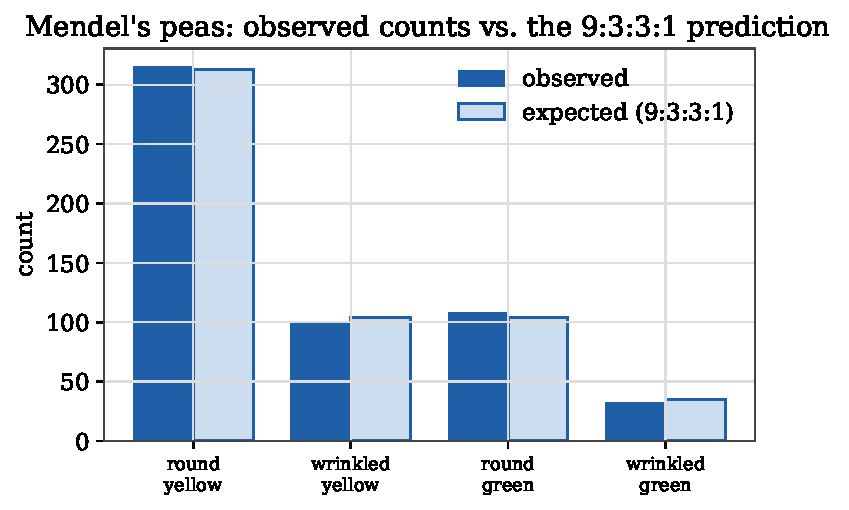
\includegraphics[width=0.55\linewidth]{mendel}
  \caption{Mendel's observed pea counts against the $9:3:3:1$ prediction. The
  near-perfect agreement is reflected in a tiny chi-square statistic.}
  \label{fig:mendel}
\end{figure}

\section{Goodness of Fit with Estimated Parameters}

Often the model under test is not fully specified—we hypothesize a Poisson
distribution but must estimate its mean from the data. Each parameter estimated
costs one further degree of freedom.

\begin{example}[Are accidents Poisson?]
The number of accidents per week at an intersection over $n=50$ weeks was:
\[
\begin{array}{c|cccc}
x & 0 & 1 & 2 & \ge 3\\\hline
\text{frequency} & 32 & 12 & 6 & 0
\end{array}
\]
Test whether the weekly count is Poisson.

\solution Under $H_0$ the count is $\Pois(\mu)$ with $\mu$ unknown. Its MLE is the
total accidents over total weeks, $\hat\mu=24/50=0.48$. Pooling into the three
categories $X=0$, $X=1$, $X\ge 2$, the estimated probabilities are
\[
  \hat p_1=e^{-0.48}=0.619,\quad \hat p_2=0.48e^{-0.48}=0.297,\quad \hat p_3=1-\hat p_1-\hat p_2=0.084,
\]
giving expected counts $E_1=30.95$, $E_2=14.85$, $E_3=4.20$. Then
\[
  t=\frac{(32-30.95)^2}{30.95}+\frac{(12-14.85)^2}{14.85}+\frac{(6-4.20)^2}{4.20}=1.354.
\]
With $k=3$ categories we lose one degree of freedom to the constraint
$\sum X_j=n$ and \emph{another} to estimating $\mu$, leaving $k-2=1$. The
$p$-value is $\Prob(\chi^2_1>1.354)=0.24$, so we do not reject $H_0$: the data
are consistent with a Poisson model for the accident counts.
\end{example}

\bigskip
This brings our tour full circle. We began by describing data, built the
probability theory to model it, and developed the inferential tools—estimation,
regression, and testing—to draw conclusions from it. Goodness-of-fit testing
closes the loop, letting us ask of any model the most basic question of all:
does it fit?


\end{document}
